\section{RoomAir Models}\label{roomair-models}

The group of models described in this section is used to account for non-uniform room air temperatures that may occur within the interior air volume of a zone. These models are accessed using the RoomAirModelType input object. RoomAir modeling was added to EnergyPlus starting with Version 1.2. Although there are many types of analyses (comfort, indoor air quality, etc) that might benefit from localized modeling of how room air varies across space, most of the room air models in EnergyPlus only address the distribution of \emph{temperature} within the zone. This allows surface heat transfer and air system heat balance calculations to be made taking into account natural thermal stratification of air and different types of intentional air distribution designs such as under-floor and side-wall displacement ventilation that purport to extract room air at higher-than-mean temperatures. The exception is the RoomAirflowNetwork model, which integrates the AirflowNetwork model and applies the nodal airflow model within zones. Note that EnergyPlus does \textbf{not} have completely general methods of modeling room air that are applicable to every conceivable type of airflow that might occur in a zone. Such models (e.g. RANS-CFD) are too computationally expensive to use with EnergyPlus for the foreseeable future. The models that are available in EnergyPlus offer only limited modeling capabilities for select room airflow configurations. Also note that because the complete mixing model for room air has long been the standard in building energy simulation, there is not currently a consensus on how to best model non-uniform air temperatures in buildings. Therefore, it is up to the user to have a good understanding of when, where, and how to apply the room air models available in EnergyPlus. The rest of this section provides some guidance in the way of examples and further discussion of the models available in EnergyPlus.

EnergyPlus offers the different types of air models listed in the table below along with the input objects associated with the use of that model.

% table 43
\begin{longtable}[c]{p{1.5in}p{1.5in}p{3.0in}}
\caption{Summary of room air models available in EnergyPlus \label{table:summary-of-room-air-models-available-in}} \tabularnewline
\toprule 
Air model name & Applicability & Input Objects Required \tabularnewline
\midrule
\endfirsthead

\caption[]{Summary of room air models available in EnergyPlus} \tabularnewline
\toprule 
Air model name & Applicability & Input Objects Required \tabularnewline
\midrule
\endhead

Well-Mixed & All zones & None, default \tabularnewline
User Defined & Any zone where the user has prior knowledge of the temperature pattern & ‘RoomAirModelType’, ‘RoomAir:TemperaturePattern:UserDefined’, ‘RoomAir:TemperaturePattern: xx’ \tabularnewline
One-Node Displacement Ventilation (Mundt) & displacement ventilation in typical office-type zones & ‘RoomAirModelType’, ‘RoomAirSettings:OneNodeDisplacementVentilation’, ‘RoomAir:Node’’ \tabularnewline
Three-Node Displacement Ventilation (UCSD) & displacement ventilation & ‘RoomAirModelType’, ‘RoomAirSettings:ThreeNodeDisplacementVentilation’ \tabularnewline
Under-Floor Air Distribution Interior Model (UCSD) & Interior zones served by a UFAD system & ‘RoomAirModelType’, ‘RoomAirSettings:UnderFloorAirDistributionInterior’ \tabularnewline
Under-Floor Air Distribution Exterior Model (UCSD) & Exterior zones served by a UFAD system & ‘RoomAirModelType’, ‘RoomAirSettings:UnderFloorAirDistributionExterior’ \tabularnewline
UCSD Cross Ventilation & cross ventilation & ‘RoomAirModelType’, ‘RoomAirSettings:CrossVentilation’ \tabularnewline
RoomAirflowNetwork & Room air model using AirflowNetwork & ‘RoomAirModelType’, ‘RoomAirSettings:AirflowNetwork’ ‘RoomAirflowNetwork:Node’, ‘RoomAirflowNetwork:Node:AdjacentSurfaceList’, ‘RoomAirflowNetwork:Node:InternalGains’, ‘RoomAirflowNetwork:Node:InternalGains’, ‘AirflowNetwork:IntraZone:Node’, ‘AirflowNetwork:IntraZone:Linkage’ \tabularnewline
\bottomrule
\end{longtable}

The room air models are coupled to the heat balance routines using the framework described by Griffith and Chen (2004).~ Their framework was modified to include features needed for a comprehensive program for annual energy modeling rather than one for hourly load calculations.~ The formulation is largely shifted from being based on the setpoint temperature to one based on the current mean air temperature.~ This is necessary to allow for floating temperatures and dual setpoint control where there may be times that the mean zone temperatures are inside the dead band.~ The coupling framework was also extended to allow for exhaust air flows (e.g.~bathroom exhaust fans) in addition to air system return flows.

The inside face temperature calculation is modified by rewriting the zone air temperature, \emph{T\(_{a}\)}, with an additional subscript, \emph{i}, for the surface index (\({T_{{a_j}}} \to {T_{{a_{i,j}}}}\) or \({T_{{a_{}}}} \to {T_{{a_i}}}\) ).~ The inside face heat balance is solved for its surface temperature using,

{\scriptsize
\begin{equation}
{T_{{s_{i,j}}}} = \frac{{{T_{s{o_{i,j}}}}{Y_{i,o}} + \sum\limits_{k = 1}^{nz} {{T_{s{o_{i,j - k}}}}} {Y_{i,k}} - \sum\limits_{k = 1}^{nz} {{T_{{s_{i,j - k}}}}} {Z_{i,k}} + \sum\limits_{k = 1}^{nq} {{\Phi_{i,k}}{{q''}_{k{i_{i,j - k}}}} + {T_{{a_{i,j}}}}{h_{{c_{i,j}}}} + {{q''}_{LWS}} + {{q''}_{LWX}} + {{q''}_{SW}} + {{q''}_{sol}}} }}{{{Z_{i,o}} + {h_{{c_{i,j}}}}}}
\end{equation}}

where:

\emph{T\(_{s}\)} is the inside face temperature

\emph{i} is the subscript indicates individual surfaces

\emph{j} is the subscript indicates current time step

\emph{k} is the subscript indicates time history steps

\emph{T\(_{so}\)} is the outside face temperature

\emph{Y\(_{i}\)} are the cross CTF coefficients

\emph{Z\(_{i}\)} are the inside CTF coefficients

\(\varphi_{i}\) are the flux CTF coefficients

\({q''_{ki}}\) is the conduction heat flux through the surface

\({h_{{c_i}}}\) is the surface convection heat transfer coefficient

\emph{T\(_{a}\)} is the near-surface air temperature

\({q''_{LWS}}\) is the longwave radiation heat flux from equipment in zone

\({q''_{LWX}}\) is the net long wavelength radiation flux exchange between zone surfaces

\({q''_{SW}}\) is the net short wavelength radiation flux to surface from lights

\({q''_{sol}}\) is the absorbed direct and diffuse solar (short wavelength) radiation.

\subsection{User Defined RoomAir Temperatures}\label{user-defined-roomair-temperatures}

The input object RoomAir:TemperaturePattern:UserDefined provides a capabity for users to define the sort of air temperature pattern he or she expects in the zone. With these models, the pattern is generally set beforehand and does not respond to conditions that evolve during the simulation.~ (Exception: the pattern available through the RoomAir:TemperaturePattern:TwoGradient object will switch between two different pre-defined vertical gradients depending on the current value of certain temperatures or thermal loads. )

The user-defined patterns obtain the mean air temperature, \({T_{MAT}}\), from the heat balance domain and then produce modified values for:

\begin{itemize}
\item \({T_{ai}}\) is the adjacent air temperature which is then used in the calculation of inside face surface temperature during the heat balance calculations.
\item \({T_{leaving}}\) is the temperature of air leaving the zone and entering the air system returns.
\item \({T_{exhaust}}\) is the temperature of air leaving the zone and entering the exhaust.
\item \({T_{stat}}\) is the temperature of air ``sensed'' at the thermostat (not currently used in air system control because air system flows use load-based control).
\end{itemize}

The user defined room air models used indirect coupling so that the patterns provide values for, or ways to calculate, how specific temperatures differ from \({T_{MAT}}\).~ The various \(\Delta T\) values determined from the model are applied to \({T_{MAT}}\) as follows:

\begin{equation}
{T_{ai}} = \Delta {T_{ai}} + {T_{MAT}}
\end{equation}

(where ``\emph{i's''} represents each surface in the zone that is affected by the model)

\begin{equation}
{T_{leaving}} = \Delta {T_{return}} + {T_{MAT}}
\end{equation}

\begin{equation}
{T_{exhaust}} = \Delta {T_{exhaust}} + {T_{MAT}}
\end{equation}

\begin{equation}
{T_{stat}} = \Delta {T_{stat}} + {T_{MAT}}
\end{equation}

The patterns defined by the object `RoomAir:TemperaturePattern:SurfaceMapping' are fairly straightforward.~ The user directly inputs values for \(\Delta {T_{ai}}\) for each surface.~ The pattern ``maps'' specific surfaces, identified by name, to \(\Delta {T_{ai}}\) values.~ This provides completely general control (but in practice may be cumbersome to use).~ The other patterns focus on temperature changes in the vertical direction.~ Surfaces do not need to be identified, but all the surfaces with the same height will be assigned the same \(\Delta {T_{ai}}\) values.

The patterns defined by the object `RoomAir:TemperaturePattern:NondimensonalHeight' apply a temperature profile based on a non-dimensionalized height, \({\rm Z}\).~ The height of each surface is defined to be the z-coordinate of the surface's centroid relative to the average z-coordinate of the floor surfaces.~ The zone ceiling height is used as the length scale to non-dimensionalize each surface's height so that,

\begin{equation}
{{\rm Z}_i} = ({z_{i,centroid}} - {z_{floorAvg}})/Ceiling\;Height
\end{equation}

(where ``\emph{i's''} represents each surface in the zone that is affected by the model)

The values for \({Z_i}\) are constrained to be between 0.01 and 0.99 because the value is meant to describe the air layer near the surface (say approximate 0.1 m from the surface) rather than the surface itself.

The user-defined profile is treated as a look up table or piecewise linear model.~ The values for \(\Delta {T_{ai}}\) are determined by searching the \({\rm Z}\) values in the user-defined profile and performing linear interpolation on the associated \(\Delta {T_a}\) values.

The patterns defined by the object `RoomAir:TemperaturePattern:ConstantGradient' apply a constant temperature gradient in the vertical direction.~ The model assumes that \({T_{MAT}}\) occurs at the mid-plane so that \({{\rm Z}_{{T_{MAT}}}} = 0.5\) (by definition).~ The surface \({Z_i}\) values are compared to \({Z_{{T_{MAT}}}}\) and then scaled with zone ceiling height to obtain values for the change in height (in units of meters), \(\Delta z\).~ The user defined gradient, \(grad\), (units of \(^{\circ}\)C/m) is then used to determine \(\Delta {T_{ai}}\) values using:

\begin{equation}
\Delta {T_{ai}} = \Delta z * grad
\end{equation}

The patterns defined by the object `RoomAir:TemperaturePattern:TwoGradient' are very similar to the constant gradient pattern above but the value of \(grad\) used at any given time is selected by interpolating between two user-defined values for \(grad\).~ Five options are available, three based on temperatures and two based on thermal loads -- see the Input Output Reference.~ The user provides upper and lower bounding values.~ If the current value of the ``sensing'' variable lies between the upper and lower bounds, then \(grad\) is determined using linear interpolation.~ If the designated value is above the upper bound then the upper value for \(grad\) is used (no extrapolation).~ Similarly, if the designated value is below the lower bound, then the lower value for \(grad\) is used.~ Note that ``upper'' and ``lower'' indicate the temperature and heat rate bounds and that the values for \(grad\) do not have to follow in the same way; the \(grad\) value for the lower bound could be higher than the \(grad\) value for the upper bound (providing a something of a reverse control scheme).~ Rather than directly using \(\Delta T\) values from the user, the temperatures for the return air, exhaust and thermostat are determined based on user-entered heights (in units of meters from the floor) and applying the current value for \(grad\).

\subsection{One-Node Displacement Ventilation RoomAir Model}\label{one-node-displacement-ventilation-roomair-model}

The input object RoomAirSettings:OneNodeDisplacementVentilation provides a simple model for displacement ventilation.~ Mundt (1996) points out that a floor air heat balance provides a simple and reasonably accurate method of modeling the temperature near the floor surface. The slope of a linear temperature gradient can then be obtained by adding a second upper air temperature value that comes from the usual overall air system cooling load heat balance.~ The figure below diagrams the temperature distribution versus height being calculated by the model.~ Mundt's floor air heat balance is extended to include convection heat gain from equipment and by ventilation or infiltration that may be introduced near the floor in order to maintain all the terms in the air heat balance of the Heat Balance Model.~ This yields the following heat balance for a floor air node,

\begin{equation}
\rho \,{c_p}\dot V({T_{AirFloor}} - {T_{Supply}}) = {h_{cFloor}}{A_{Floor}}({T_{Floor}} - {T_{AirFloor}}) + {Q_{ConvSourceFloor}} + {Q_{InfilFloor}}
\end{equation}

where:

\emph{\(\rho\)} is the air density

\emph{c\(_{p}\)} is the air specific heat at constant pressure

\(\mathop V\limits^\cdot\) is the air system flow rate

\emph{T\(_{supply}\)} is the air system's supply air drybulb temperature

\emph{h\(_{cFloor}\)} ~is the convection heat transfer coefficient for the floor

\emph{A\(_{floor}\)} is the surface area of the floor

\emph{T\(_{floor}\)} is the surface temperature of the floor

\emph{Q\(_{convSourceFloor}\)} is the convection from internal sources near the floor (\textless{} 0.2 m)

\emph{Q\(_{InfilFloor}\)} is the heat gain (or loss) from infiltration or ventilation near the floor.

``Floor splits'' are the fraction of total convective or infiltration loads that are dispersed so as to add heat to the air located near the floor.~ The user prescribes values for floor splits as input.~ No guidance is known to be available to use in recommending floor splits, but the user could for example account for equipment known to be near the floor, such as tower computer cases, or supplementary ventilation designed to enter along the floor.~ The equation above can be solved directly for \emph{T\(_{AirFloor}\)} and is used in the form of the equation below,

\begin{equation}
{T_{AirFloor}} = \frac{{\rho \,{c_p}\dot V{T_{Supply}} + \sum {{h_{cFloor}}{A_{Floor}}{T_{Floor}}}  + {{\dot Q}_{ConvSourceFloor}} + {{\dot Q}_{InfilFloor}}}}{{\rho \,{c_p}\dot V + \sum {{h_{cFloor}}{A_{Floor}}} }}
\end{equation}

The upper air node temperature is obtained by solving the overall air heat balance for the entire thermal zone for the temperature of the air leaving the zone and going into the air system return, \emph{T\(_{leaving}\)}.

\begin{equation}
{T_{Leaving}} = \frac{{ - {{\dot Q}_{sys}}}}{{p{c_p}\dot V}} + {T_{Supply}}
\end{equation}

where \({\dot Q_{sys}}\) is the air system heat load with negative values indicating a positive cooling load.~ Values for \({\dot Q_{sys}}\) are computed by the load calculation routines and passed to the air model.~ The vertical temperature gradient or slope, \emph{dT/dz}, is obtained from,

\begin{equation}
\frac{{dT}}{{dz}} = \frac{{{T_{Leaving}} - {T_{AirFloor}}}}{{{H_{return}}}}
\end{equation}

where \emph{H\(_{return}\)} is the distance between the air system return and the floor air node assumed to be 0.1 m from the floor and \emph{z} is the vertical distance.

\begin{figure}[hbtp] % fig 132
\centering
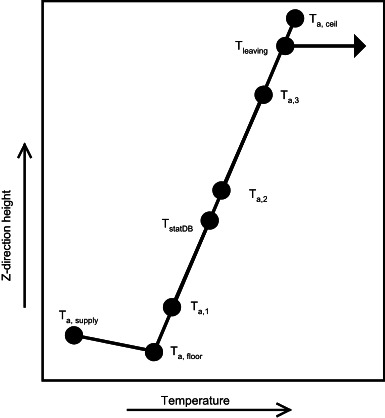
\includegraphics[width=0.9\textwidth, height=0.9\textheight, keepaspectratio=true]{media/image2341.svg.png}
\caption{Height versus temperature schematic for Mundt model \protect \label{fig:height-versus-temperature-schematic-for-mundt}}
\end{figure}

The constant slope allows obtaining temperatures at any vertical location using,

\begin{equation}
{T_{{a_i}}} = {T_{leaving}} - \frac{{dT}}{{dz}}({z_{leaving}} - {z_i})
\end{equation}

So for example the temperatures near the ceiling can easily be determined. Accounting for the location of the thermostat inside the zone (e.g.~1.1 m) is accomplished by returning the temperature for the appropriate height to the appropriate air node used for control. If the walls are subdivided in the vertical direction as shown in the figure above, then the air model can provide individual values for each surface based on the height and slope.~ However, no additional heat balances are necessarily made (in the air domain) at these points as all the surface convection is passed to the model in the totaled value for \({\dot Q_{sys}}\).

\subsection{Three-Node Displacement Ventilation RoomAir Model}\label{three-node-displacement-ventilation-roomair-model}

\subsubsection{Overview}\label{overview-005}

The input object RoomAirSettings:ThreeNodeDisplacementVentilation provides a simple model for heat transfer and vertical temperature profile prediction in displacement ventilation. The fully-mixed room air approximation that is currently used in most whole building analysis tools is extended to a three node approach, with the purpose of obtaining a first order precision model for vertical temperature profiles in displacement ventilation systems. The use of three nodes allows for greatly improved prediction of thermal comfort and overall building energy performance in low energy cooling strategies that make use of unmixed stratified ventilation flows.

The UCSD Displacement Ventilation Model is one of the non-uniform zone models provided through the Room Air Manager in EnergyPlus. The intent is to provide a selection of useful non-uniform zone air models to enable the evaluation of air-conditioning techniques that use stratified or partially stratified room air. Such techniques include displacement ventilation (DV) and underfloor air distribution (UFAD) systems. The methodology can also include, in principle, natural displacement ventilation and also wind-driven cross-ventilation (CV).

\subsubsection{Displacement Ventilation}\label{displacement-ventilation}

A DV system is a complete contrast to a conventional forced air system. In a conventional system conditioned air is delivered at ceiling level and the intent is to create a fully mixed space with uniform conditions. In a DV system conditioned air is delivered at floor level and low velocity in order to minimize mixing and to establish a vertical temperature gradient. The incoming air ``displaces'' the air above it which, in turn,~ is exhausted through ceiling level vents. In DV a noticeable interface occurs between the occupied zone of the room and a mixed hot layer near the ceiling of the room(Dominique \& Guitton, 1997). Maintaining the lower boundary of this warm layer above the occupied zone is one of the many unique challenges of displacement ventilation design. Often DV systems use 100\% outside air. The vertical displacement air movement means that convective heat gains introduced near the ceiling will be removed without affecting the occupied region of the room. Also a fraction of the heat gains that occur in the occupied zones rise as plumes into the upper part of the space, thereby reducing the cooling load. Similarly the fresh air will be used more effectively than with a fully mixed system: the fresh air won't be ``wasted'' in the upper, unoccupied region of the room. Finally, the vertical temperature gradient means that the average room temperature can be higher for a DV conditioned room than with a conventionally conditioned room: the occupants feel the lower temperature in the lower region of the room and are unaffected by the higher temperature near the ceiling. However, whenever the outside air temperature is above \(\approx\)19\(^{\circ}\)C this advantage is mostly lost: the internal loads must be removed from the space independently of the airflow pattern (during the warmer hours buildings tend to be almost closed to the outside, operating in closed loop). The inflow temperature advantage is then only useful for the minimum outside air that must always be provided (in most cases this remaining advantage is negligible).

DV systems have limitations. In order to avoid chilling the occupants the supply air temperature used for DV is considerably higher than that used in conventional forced-air systems. This can lead to problems in removing both sensible and latent loads. Exterior spaces may have conditions that are not conducive to establishing a vertical temperature gradient. DV systems seem to be best suited to interior spaces with only moderate loads.

\subsubsection{Non-uniform zone models}\label{non-uniform-zone-models}

Several types of models have been proposed as suitable for inclusion in building energy simulation (BES) programs. These models must be simple enough not to impose an undue computational burden on a BES program, yet provide enough predictive capability to produce useful comparisons between conventional and stratified zone operation strategies. ASHRAE RP-1222 (Chen \& Griffith 2002) divides the candidate models into two categories: \emph{nodal} and \emph{zonal}. Nodal models describe the zone air as a network of nodes connected by flow paths; each node couples convectively to one or more surfaces. Zonal models are coarse--grained finite volume models. ASHRAE RP-1222 provides a short history (and examples) of each type of model. In terms of nodal models for displacement ventilation we mention the Mundt model (Mundt 1996), since it is implemented in EnergyPlus, and the Rees-Haves model (Rees \& Haves 2001) since it is a well developed nodal-type model and is implemented in the RP-1222 toolkit. The Rees-Haves model, while successful in predicting the flow and temperature field for geometries similar to those used in its development, can suffer from lack of flexibility and clarity in the modeling approximations. When dealing with diverse geometries it is not clear that the flow coefficients used in the model are applicable or why they can be used since plumes, the fundamental driving mechanisms of the displacement flow, are not explicitly modeled. This is the main difference between the DV models implemented in theRP-1222 toolkit and the model that is described here.

The UCSD DV model is closer to a nodal model than to a zonal model. However, it is best to classify it in a separate category: plume equation based multi-layer models (Linden \emph{et al}. 1990, Morton \emph{et al}. 1956). These models assume that the dominant mechanism is plume-driven flow from discrete internal sources and that other effects (such as buoyancy driven flow at walls or windows) may be neglected. Alternatively, these heat sources also produce plumes that can be included in the model. The result is a zone divided vertically into two or more well separated regions -- each region characterized by a single temperature or temperature profile. This characterization allows the physics of the heat gains and the ventilation flow to be represented in a realistic manner, without the introduction of \emph{ad hoc} assumptions.

\subsubsection{Model Description}\label{model-description-002}

\subsubsection{Single Plume Two Layer Model}\label{single-plume-two-layer-model}

The simplest form of the plume equation based models is the case of a single plume in an adiabatic box with constant supply air flow. For this configuration two layers form in the room: a lower layer with similar density and temperature as the inflow air and a mixed upper layer with the same density / temperature as the outflow air. The main assumption of this model, successfully validated against scaled model experiments (Linden \emph{et al.} 1990), is that the interface between the two layers occurs at the height (h) where the vertical buoyancy driven plume flow rate is the same as the inflow rate. For a point source of buoyancy in a non-stratified environment (a plume) the airflow rate increases with vertical distance from the source according to:

\begin{equation}
\dot V = C\cdot {B^{1/3}}{z^{5/3}}
\end{equation}

where:

\(\dot V\) = plume volume flux {[}m3/s{]}

\(B\) = buoyancy flux~ {[}m4/s3{]}

\(z\) = vertical distance above source {[}m{]}

\begin{equation}
C = \frac{6}{5}\alpha {(\frac{9}{{10}}\alpha )^{1/3}}{\pi ^{2/3}}
\end{equation}

\(\alpha\) = plume entrainment constant; a value of~ 0.127 is used, suitable for top-hat profiles for density and velocity across the plumes.

For an ideal gas:

\begin{equation}
\Delta \rho /\rho  = \Delta {\rm T}/{\rm T}
\end{equation}

resulting in the following relation between heat input rate and buoyancy flux:

\begin{equation}
B = \frac{{g\dot Q}}{{\rho {C_p}T}}
\end{equation}

where

\(\rho\) = density of air {[}kg/m3{]}

\(T\) = air temperature {[}K{]}

\(g\) = acceleration of gravity {[}m/s2{]}

\(\dot Q\) = heat input rate {[}W{]}

\({C_p}\) = specific heat capacity of air {[}J/kgK{]}

Since the plume volume flow rate increases with height with exponent 5/3, for any room inflow rate (F, (m\(^{3}\)/s)) there will always be a height (h,(m)) where the plume driven flow rate matches the inflow rate. This height is obtained by setting (1.1) equal to F and solving for z = h:

\begin{equation}
h = {F^{3/5}}/({C^{3/5}}{B^{1/5}})
\end{equation}

Substituting in and introducing air properties at 20\(^{\circ}\)C gives:

\begin{equation}
h = 24.55\cdot {F^{3/5}}/{\dot Q^{1/5}}
\end{equation}

\subsubsection{Multiple Plumes and Wall Heat Transfer}\label{multiple-plumes-and-wall-heat-transfer}

Of course, it would be rare for a real world case to consist of a single point-source plume originating on the floor, unaffected by heat gains from walls and windows. For multiple plumes of equal strength a straight-forward extension of the single is possible. N plumes of unequal strength result in the formation of n vertical layers. This case is much more complex but if we are satisfied with a first order precision model the equal strength model can be used by averaging the plume strengths (Carrilho da Graça, 2003). Even in a case where all plumes are of equal strength, nearby plumes may coalesce. Plumes that are less than 0.5 meters apart at their source will coalesce within 2 meters (Kaye \& Linden,2004).

As the complexity of the physical systems modeled increases some limitations must be imposed. In particular, the biggest challenge remains the interaction between wall driven boundary layers (positively and negatively buoyant) and displacement flows. For this reason, the model that is developed below is not applicable when:

\begin{enumerate}
\item Downward moving buoyancy driven airflow rate is of the same order of magnitude as plume driven flow (these airflow currents are typically generated on lateral surfaces or in the ceiling whenever these surfaces are much cooler than the room air).
\item Upward moving wall or floor generated buoyancy flux in the lower layer is of the same order of magnitude as plume driven flow.
\end{enumerate}

Although these limitations are significant it is important to note that even in the presence of dominant convection from the floor surface, a buoyancy, two layer flow can be established whenever the plume buoyancy flux is more than 1/7 of the horizontal flux (Hunt \emph{et al.} 2002). A two layer structure can also originate when the only heat source is a heated portion of the room floor, as long as the heated area does not exceed 15\% of the room floor (Holford \emph{et al.} 2002).

For the case of multiple non-coalescing plumes (n), with equal strength, the total vertical airflow for a given height is:

\begin{equation}
  \dot{V} = CnB^{1/3}z^{5/3}
\end{equation}

resulting in a mixed layer height of:

\begin{equation}
  h = \frac{24.55F^{3/5}}{{n^3 \dot{Q}}^{1/5}}
\end{equation}

\subsubsection{Implementation}\label{implementation}

The model predicts three temperatures that characterize the three main levels in the stratification of the room:

\begin{enumerate}
\item A floor level temperature T\(_{floor}\) to account for the heat transfer from the floor into the supply air.
\item An occupied subzone temperature T\(_{oc}\) representing the temperature of the occupied region.
\item An upper level temperature T\(_{mx}\) representing the temperature of the upper, mixed region and the outflow temperature.
\end{enumerate}

We assume that the model for multiple, equal strength plumes (equations and will be adequate for our calculations. The supply air flow rate \(\dot V\) is obtained by summing all the air flows entering the zone: supply air, infiltration, ventilation, and inter-zone flow. The heat gain \(\dot Q\) is estimated by summing all the convective internal gains located in the occupied subzone -- task lights, people, equipment -- and dividing this power equally among the n plumes. With these assumptions we can describe the implementation.

The UCSD DV model is controlled by the subroutine \emph{ManageUCSDDVModel} which is called from the \emph{RoomAirModelManager}. The \emph{RoomAirModelManager} selects which zone model will be used for each zone.

The calculation is done in subroutine \emph{CalcUCSDDV}. First we calculate the convective heat gain going into the upper and lower regions.

\begin{equation}
\dot Q_{ocz} = \dot Q_{oc,conv} + \dot Q_{tl,conv} + \dot Q_{eleq,conv} + \dot Q_{gaseq,conv} + \dot Q_{otheq,conv} + \dot Q_{hw,conv} + \dot Q_{stmeq,conv} + \dot Q_{bb,conv}
\end{equation}

\begin{equation}
{\dot Q_{mxz}} = {\dot Q_{gl,conv}} + {\dot Q_{ltp}} + {\dot Q_{htrad,conv}}
\end{equation}

\begin{equation}
{\dot Q_{tot,conv}} = {\dot Q_{ocz}} + {\dot Q_{mxz}}
\end{equation}

Next we sum up the inlet air flows in the form of MCP (mass flow rate times the air specific heat capacity) and MCPT (mass flow rate times C\(_{p}\) times air temperature).

\begin{equation}
MC{P_{zone}} = MC{P_i} + MC{P_{vent}} + MC{P_{mix}}
\end{equation}

\begin{equation}
MC{P_{sys}} = \sum\limits_{inlets} {{{\dot m}_i}} {C_{p,i}}
\end{equation}

\begin{equation}
MC{P_{tot}} = MC{P_{zone}} + MC{P_{sys}}
\end{equation}

\begin{equation}
MCP{T_{zone}} = MCP{T_i} + MCP{T_{vent}} + MCP{T_{mix}}
\end{equation}

\begin{equation}
MCP{T_{sys}} = \sum\limits_{inlets} {{{\dot m}_i}} {C_{p,i}}{T_i}
\end{equation}

\begin{equation}
MCP{T_{tot}} = MCP{T_{zone}} + MCP{T_{sys}}
\end{equation}

The number of plumes per occupant \({N_{plumesperpers}}\) is a user input. The total number of plumes in the zone is:

\begin{equation}
{N_{plumes}} = {N_{occ}} \cdot {N_{plumesperperson}}
\end{equation}

The gains fraction \(F{r_{gains}}\) is a user input via a schedule. It is the fraction of the convective gains in the occupied subzone that remain in that subzone. Using this we calculate the total power in the plumes and the power per plume.

\begin{equation}
{\dot Q_{plumes}} = (1 - F{r_{gains}}) \cdot {\dot Q_{tot,conv}}
\end{equation}

\begin{equation}
{\dot Q_{perplume}} = {\dot Q_{plumes}}/{N_{plumes}}
\end{equation}

We now make an initial estimate of the height fraction \emph{Fr\(_{hb}\)} (height of the boundary layer divided by the total zone height).

\begin{equation}
F{r_{hb}} = \left( {{{24.55} \mathord{\left/ {\vphantom {{24.55} {{H_{ceil}}}}} \right. } {{H_{ceil}}}}} \right){\left( {\frac{{0.000833 \cdot MC{P_{tot}}}}{{{N_{plumes}} \cdot \dot Q_{perplume}^{1/3}}}} \right)^{3/5}}
\label{eq:RoomAirHeightBoundaryLayer}
\end{equation}

where 0.000833~ = \(1/({\rho_{air}} \cdot {c_{p,air}})\) converts \(MC{P_{tot}}\) to a volumetric flow rate. Next we iterate over the following 3 steps.

\subsubsection{Iterative procedure}\label{iterative-procedure}

\begin{enumerate}
\item Call subroutine \emph{HcUCSDDV} to calculate a convective heat transfer coefficient for each surface in the zone, an effective air temperature for each surface, and HA\(_{mx}\), HAT\(_{mx}\), HA\(_{oc}\), HAT\(_{oc}\), HA\(_{fl}\), and HAT\(_{fl}\). Here HA is \(\sum\limits_{surfaces} {{h_{c,i}}} \cdot {A_i}\) ~for a region and HAT is \(\sum\limits_{surfaces} {{h_{c,i}}} \cdot {A_i} \cdot {T_i}\) ~for a region. The sum is over all the surfaces bounding the region; \({h_{c,i}}\) ~is the convective heat transfer coefficient for surface i, \({A_i}\) ~is the area of surface i,~ and \({T_i}\) ~is the surface temperature of surface i.
\item Recalculate \(F{r_{hb}}\) using the Equation~\ref{eq:RoomAirHeightBoundaryLayer}.
\item Calculate the three subzone temperatures: \emph{T\(_{fl,}\) T\(_{oc}\)} and \emph{T\(_{mx}\)}.
\end{enumerate}

The h\(_{c}\)'s calculated in step 1 depend on the subzone temperatures and the boundary layer height. In turn the subzone temperatures depend on the HA and HAT's calculated in step 1. Hence the need for iteration

Next we describe Steps 1 and 3 in more detail.

\subsubsection{Step 1}\label{step-1}

Subroutine \emph{HcUCSDDV} is quite straightforward. It loops through all the surfaces in each zone and decides whether the surface is located in the upper, mixed subzone or the lower, occupied subzone, or if the surface is in both subzones. If entirely in one subzone the subzone temperature is stored in the surface effective temperature variable \emph{SurfTempEffBulkAir(SurfNum)} and h\(_{c}\) for the surface is calculated by a call to subroutine \emph{CalcDetailedHcInForDVModel}. This routine uses the ``detailed'' natural convection coefficient calculation that depends on surface tilt and \(\Delta {T^{1/3}}\). This calculation is appropriate for situations with low air velocity.

For surfaces that bound 2 subzones, the subroutine calculates h\(_{c}\) for each subzone and then averages them, weighting by the amount of surface in each subzone.

During the surface loop, once the h\(_{c}\)~for a surface is calculated, the appropriate subzone HA and HAT sums are incremented. If a surface is in 2 subzones the HA and HAT for each subzone are incremented based on the area of the surface in each subzone.

\subsubsection{Step 3}\label{step-3}

The calculation of subzone temperatures follows the method used in the \textbf{\emph{ZoneTempPredictorCorrector}} module and described in the section \textbf{Basis for the System and Zone Integration}. Namely a third order finite difference expansion of the temperature time derivative is used in updating the subzone temperatures. Otherwise the subzone temperatures are obtained straightforwardly by solving an energy balance equation for each subzone.

{\scriptsize
\begin{equation}
T_{fl} = (C_{air,fl} \cdot (3 \cdot T_{ - 1,fl} - (3/2) \cdot T_{ - 2,fl} + (1/3) \cdot T_{ - 3,fl}) + HAT_{fl} + MCPT_{tot} + 0.6 \cdot T_{oc} \cdot MCP_{tot})  / ((11/6) \cdot C_{air,fl} + HA_{fl} + 1.6 \cdot MCP_{tot})
\end{equation}}

{\scriptsize
\begin{equation}
  \begin{array}{l}
    T_{oc} = (C_{air,oc} \cdot (3 \cdot T_{ - 1,oc} - (3/2) \cdot T_{ - 2,oc} + (1/3) \cdot T_{ - 3,oc}) + \dot Q_{ocz} \cdot Fr_{gains} + HAT_{oc} + 1.6 \cdot T_{fl} \cdot MCP_{tot}) \\
    / ((11/6) \cdot C_{air,oc} + HA_{oc} + 1.6 \cdot MCP_{tot})
\end{array}
\end{equation}}

{\scriptsize
\begin{equation}
  \begin{array}{l}
    T_{mx} = (C_{air,mx} \cdot (3 \cdot T_{ - 1,mx} - (3/2) \cdot T_{ - 2,mx} + (1/3) \cdot T_{ - 3,mx}) + \dot Q_{ocz} \cdot (1 - Fr_{gains}) + \dot Q_{mxz} + HAT_{mx} + T_{oc} \cdot MCP_{tot}) \\
    / ((11/6) \cdot C_{air,mx} + HA_{mx} + MCP_{tot})
  \end{array}
\end{equation}}

Here \({C_{air,fl}}\), \({C_{air,oc}}\), and \({C_{air,mx}}\) are the heat capacities of the air volume in each subzone.~ \({C_{air,mx}}\) is calculated by:

\begin{equation}
{R_{air,mx}} = {V_{mx}} \cdot (\Delta {z_{mx}}/{z_{ceil}}) \cdot {\rho_{air,mx}} \cdot {c_{p,air,mx}} \cdot Mu{l_{cap}}/(\Delta {t_z} \cdot 3600)
\end{equation}

\begin{equation}
{C_{air,mx}} = {R_{air,mx}} \cdot \Delta {t_z}/\Delta {t_{sys}}
\end{equation}

The other subzone air heat capacities are calculated in the same manner.

\subsubsection{Mixed calculation}\label{mixed-calculation}

The above iterative procedure assumed that displacement ventilation was taking place: i.e., conditions were favorable temperature stratification in the zone. Now that this calculation is complete and the subzone temperatures and depths calculated, we check to see if this assumption was justified. If not, zone conditions must be recalculated assuming a well-mixed zone.

If \({T_{mx}} < {T_{oc}}\) or \(MC{P_{tot}} \le 0\) or \({H_{fr}} \cdot {H_{ceil}} < {H_{fl,top}} + \Delta {z_{occ,\min }}\) then the following mixed calculation will replace the displacement ventilation calculation.

\textbf{Note:} ~\(\Delta {z_{occ,\min }}\) is the minimum thickness of occupied subzone. It is set to 0.2 meters. \({H_{fl,top}}\) is the height of the top of the floor subzone. It is defined to be 0.2 meters; that is, the floor subzone is always 0.2 meters thick and \({T_{fl}}\) ~is the temperature at 0.1 meter above the floor surface.

The mixed calculation iteratively calculates surface convection coefficients and room temperature just like the displacement ventilation calculation described above. In the mixed case however, only one zone temperature \emph{T\(_{avg}\)} is calculated. The 3 subzone temperatures are then set equal to \emph{T\(_{avg}\)}.

First, \emph{Fr\(_{hb}\)} is set equal to zero.

Then the code iterates over these steps.

1.~Calculate \emph{T\(_{avg}\)} using:

{\scriptsize
\begin{equation}
\begin{array}{l}
T_{avg} = (C_{air,z} \cdot (3 \cdot T_{ - 1,z} - (3/2) \cdot T_{ - 2,z} + (1/3) \cdot T_{ - 3,z}) + \dot Q_{tot,conv} + HAT_{oc} + HAT_{mx} + HAT_{fl} + MCPT_{tot}) \\
\quad \quad \quad \quad / ((11/6) \cdot C_{air,z} + HA_{oc} + HA_{mx} + HA_{fl} + MCP_{tot})
\end{array}
\end{equation}}

\begin{equation}
{T_{mx}} = {T_{avg}}
\end{equation}

\begin{equation}
{T_{oc}} = {T_{avg}}
\end{equation}

\begin{equation}
{T_{fl}} = {T_{avg}}
\end{equation}

2.~Call \emph{HcUCSDDV} to calculate the \emph{h\(_{c}\)}'s.

3.~Repeat step 1

\subsubsection{Final calculations}\label{final-calculations}

The displacement ventilation calculation finishes by calculating some report variables. Using Equation~\ref{eq:RoomAirHeightBoundaryLayer}, setting the boundary height to 1.5 meters and solving for the flow, we calculate a minimum flow fraction:

\begin{equation}
{\dot V_{\min }} = {(1.5/{\rm{24}}{\rm{.55)}}^{{\rm{5/3}}}} \cdot {N_{plumes}} \cdot \dot Q_{perplume}^{1/3}
\end{equation}

\begin{equation}
F{r_{\min flow}} = .000833 \cdot MC{P_{tot}}/{\dot V_{\min }}
\end{equation}

We define heights:

\begin{equation}
{H_{trans}} = F{r_{hb}} \cdot {H_{ceil}}
\end{equation}

\begin{equation}
{H_{mxavg}} = ({H_{ceil}} + {H_{trans}})/2
\end{equation}

\begin{equation}
{H_{ocavg}} = ({H_{fltop}} + {H_{trans}})/2
\end{equation}

\begin{equation}
{H_{flavg}} = {H_{fltop}}/2
\end{equation}

Using the user defined comfort height we calculate the comfort temperature.

If mixing:

\begin{equation}
{T_{comf}} = {T_{avg}}
\end{equation}

If displacement ventilation:

If \emph{H\(_{comf}\)} \textless{} \emph{H\(_{flavg}\)}:

\begin{equation}
{T_{comf}} = {T_{fl}}
\end{equation}

Else if \({H_{comf}} \ge {H_{flavg}}\) ~and \({H_{comf}} < {H_{ocavg}}\):

\begin{equation}
{T_{comf}} = ({T_{fl}}({H_{ocavg}} - {H_{comf}}) + {T_{mx}}({H_{comf}} - {H_{flavg}})/({H_{ocavg}} - {H_{flavg}})
\end{equation}

Else if \({H_{comf}} \ge {H_{ocavg}}\) ~and \({H_{comf}} < {H_{mxavg}}\):

\begin{equation}
{T_{comf}} = ({T_{oc}}({H_{mxavg}} - {H_{comf}}) + {T_{mx}}({H_{comf}} - {H_{ocavg}})/({H_{mxavg}} - {H_{ocavg}})
\end{equation}

Else if \({H_{comf}} \ge {H_{mxavg}}\) ~and \({H_{comf}} < {H_{ceil}}\):

\begin{equation}
{T_{comf}} = {T_{mx}}
\end{equation}

Using the user defined thermostat height we calculate the temperature at the thermostat.

If mixing:

\begin{equation}
{T_{stat}} = {T_{avg}}
\end{equation}

If displacement ventilation:

If \emph{H\(_{stat}\)} \textless{} \emph{H\(_{flavg}\)}:

\begin{equation}
{T_{stat}} = {T_{fl}}
\end{equation}

Else if \({H_{stat}} \ge {H_{flavg}}\) ~and \({H_{stat}} < {H_{ocavg}}\):

\begin{equation}
{T_{stat}} = ({T_{fl}}({H_{ocavg}} - {H_{stat}}) + {T_{mx}}({H_{stat}} - {H_{flavg}})/({H_{ocavg}} - {H_{flavg}})
\end{equation}

Else if \({H_{stat}} \ge {H_{ocavg}}\) ~and \({H_{stat}} < {H_{mxavg}}\):

\begin{equation}
{T_{stat}} = ({T_{oc}}({H_{mxavg}} - {H_{stat}}) + {T_{mx}}({H_{stat}} - {H_{ocavg}})/({H_{mxavg}} - {H_{ocavg}})
\end{equation}

Else if \({H_{stat}} \ge {H_{mxavg}}\) ~and \({H_{stat}} < {H_{ceil}}\):

\begin{equation}
{T_{stat}} = {T_{mx}}
\end{equation}

The average temperature gradient is:

If \({H_{mxavg}} - {H_{flavg}} > 0.1\):

\begin{equation}
Grad{T_{avg}} = ({T_{mx}} - {T_{fl}})/({H_{mxavg}} - {H_{flavg}})
\end{equation}

else \(Grad{T_{avg}} =  - 9.999\)

The maximum temperature gradient is:

If~ \({H_{ocavg}} - {H_{flavg}} > 0.1\):

\begin{equation}
Grad{T_{\max ,1}} = ({T_{oc}} - {T_{fl}})/({H_{ocavg}} - {H_{flavg}})
\end{equation}

else \(Grad{T_{\max ,1}} = - 9.999\)

If~ \({H_{mxavg}} - {H_{ocavg}} > 0.1\):

\begin{equation}
Grad{T_{\max ,2}} = ({T_{mx}} - {T_{oc}})/({H_{mxavg}} - {H_{ocavg}})
\end{equation}

else \(Grad{T_{\max ,2}} = - 9.999\) and

\begin{equation}
Grad{T_{\max }} = \max (Grad{T_{\max ,1}},Grad{T_{\max ,2}})
\end{equation}

For reporting purposes, if the zone is deemed to be mixed, the displacement ventilation report variables are set to flag values.

If \({T_{mx}} < {T_{oc}}\) ~or \(MC{P_{tot}} \le 0\) ~or \({H_{fr}} \cdot {H_{ceil}} < {H_{fl,top}} + \Delta {z_{occ,\min }}\) ~or \({T_{mx}} - {T_{oc}} < \Delta {T_{Crit{\mathop{\rm Re}\nolimits} p}}\)

\begin{equation}
Grad{T_{avg}} =  - 9.999
\end{equation}

\begin{equation}
Grad{T_{\max }} =  - 9.999
\end{equation}

\begin{equation}
F{R_{\min ,flow}} =  - 1.0
\end{equation}

\begin{equation}
{H_{trans}} =  - 9.999
\end{equation}

Finally, the zone node temperature is set to \emph{T\(_{mx}\)}.

\subsection{Under-Floor Air Distribution Interior Zone Model}\label{under-floor-air-distribution-interior-zone-model}

\subsubsection{Overview}\label{overview-1-001}

The input object RoomAirSettings:UnderFloorAirDistributionInterior provides a simple model for heat transfer and nonuniform vertical temperature profile for interior zones of a UFAD system. These zones are expected to be dominated by internal loads, a portion of which (such as occupants and workstations) will act to generate plumes. The plumes act to potentially create room air stratification, depending on the type \& number of diffusers, the amount and type of load, and the system flowrate. In order to better model this situation the fully-mixed room air approximation that is currently used in most whole building analysis tools is extended to a two node approach, with the purpose of obtaining a first order precision model for vertical temperature profiles for the interior zones of UFAD systems. The use of 2 nodes allows for greatly improved prediction of thermal comfort and overall building energy performance for the increasingly popular UFAD systems.

The UCSD UFAD Interior Zone Model is one of the non-uniform zone models provided through the Room Air Manager in EnergyPlus. The intent is to provide a selection of useful non-uniform zone air models to enable the evaluation of air-conditioning techniques that use stratified or partially stratified room air. Such techniques include displacement ventilation (DV) and underfloor air distribution (UFAD) systems. The methodology can also include natural displacement ventilation and also wind-driven cross-ventilation (CV).

\subsubsection{Underfloor air distribution systems}\label{underfloor-air-distribution-systems}

UFAD systems represent, in terms of room air stratification, an intermediate condition between a well-mixed zone and displacement ventilation. Air is supplied through an underfloor plenum at low pressure through diffusers in the raised floor. The diffusers can be of various types: e.g., swirl, variable-area, displacement, and produce more or less mixing in the zone. UFAD systems are promoted as saving energy due to: higher supply air temperature; low static pressure; cooler conditions in the occupied subzone than in the upper subzone; and sweeping of some portion of the convective load (from ceiling lights, for instance) into the return air without interaction with the occupied region of the zone.

Modeling a UFAD system is quite complex and involves considerably more than just a non-uniform zone model. The zones' coupling to the supply and return plenums must be modeled accurately (particularly radiative transfer from a warm ceiling to a cool floor and on into the supply plenum by conduction). The supply plenum must be accurately modeled, giving a good estimate of the supply air temperature and conduction heat transfer between supply \& return plenums through the slab. The HVAC system must be modeled including return air bypass and various types of fan powered terminal units.

The UCSD UFAD interior zone model is similar to the UCSD DV model. The most obvious difference is that the UFAD model has no separate near-floor subzone. Like the UCSD DV model it is a plume equation based multi-layer model (2 layers in this case). The zone is modeled as being divided into 2 well separated subzones which we denote as ``occupied'' and ``upper''. Each subzone is treated as having a single temperature. The boundary between the 2 subzones moves up \& down each time step as a function of zone loads and supply air flow rate. Thus at each HVAC time step, the height of the boundary above the floor must be calculated, portions of surfaces assigned to each subzone, and a separate convective heat balance performed on each subzone.

\subsubsection{Model Description}\label{model-description-1-001}

The UFAD interior zone model is based upon non-dimensional analysis of the system and using the non-dimensional description to make a comparison between full-scale UCB test chamber data \& small-scale UCSD salt tank measurements.

In order to do the non-dimensional comparisons, we need to define two dimensionless parameters. One is \(\Gamma\), and the other is \(\phi\). Lin \& Linden (Lin \& Linden, 2005) showed that in a UFAD system, the buoyancy flux of the heat source \((B)\) and the momentum flux of the cooling jets \((M)\) are the controlling parameters on the stratification. Since \([B] = {L^4}{T^{ - 3}}\) and\([M] = {L^4}{T^{ - 2}}\) , we can have a length scale as \({M^{3/4}}/{B^{1/2}}\) .

\emph{Definition of \(\Gamma\) for the single-plume single-diffuser basic model}

We observed, in our small-scale experiments, that the total room height does not affect the interface position, or the height of the occupied zone. In other words, \emph{H} might not be the critical length scale for the stratification. Therefore, we started to use \(\sqrt A\) ~as the reference length. Then \(\Gamma\) is defined as:

\begin{equation}
\Gamma  = \frac{{{M^{3/4}}}}{{{B^{1/2}}{A^{1/2}}}} = \frac{{{{({Q^2}/A)}^{3/4}}}}{{{B^{1/2}}{A^{1/2}}}} = \frac{{{Q^{3/2}}}}{{{A^{5/4}}{B^{1/2}}}}
\label{eq:GammaSinglePlumeSingleDiffuser}
\end{equation}

\emph{Definition for multi-diffuser and multi-source cases}

We only considered single-diffuser, single-source cases in above analysis. Suppose there are \emph{n} equal diffusers and \emph{m} equal heat sources in a UFAD room. We shall divide the number of diffusers up into a number of separate heat sources so that each subsection with \emph{n' = n/m} diffusers per heat source will have the same stratification as other subsections. Further, the air flow and the heat load into the subsection \emph{Q'} and \emph{B'} will be \(Q' = Q/m\) \(B' = B/m\) respectively, where \emph{Q'} and \emph{B'} are the total air flow and the total heat load for the entire UFAD space. Then the momentum flux each diffuser per heat source carries is \({M_d} = {(\frac{1}{{n'}}Q')^2}/A\). Equation~\ref{eq:GammaSinglePlumeSingleDiffuser} will be modified as:

\begin{equation}
\Gamma  = \frac{{{{(n'{M_d})}^{3/4}}}}{{B{'^{1/2}}\sqrt {n'A} }} = \frac{{Q{'^{3/2}}}}{{{{(n'A)}^{5/4}}B{'^{1/2}}}} = \frac{{{Q^{3/2}}}}{{m{{(n'A)}^{5/4}}{B^{1/2}}}}
\label{eq:GammaMultiDiffuserMultiSource}
\end{equation}

\emph{Full-scale cases}

Because \emph{B} is the buoyancy flux of the heat sources and \emph{M} is the momentum flux of the cooling jets, in a real full-scale room, we shall consider the total room net heat load (plume heat input, minus the room losses) and the total net flow rate coming from the diffusers (input room air flow, minus the room leakage). Further, if the diffuser is swirl type, the vertical momentum flux should be used.

\begin{equation}
\Gamma  = \frac{{{{(Q\cos \theta )}^{3/2}}}}{{m{{(n'A)}^{5/4}}{{(0.0281W)}^{1/2}}}}
\label{eq:GammaFullScaleCases}
\end{equation}

where \emph{Q} is the net flow rate coming out from all diffusers (m\(^{3}\)/s); \emph{W} is the total net heat load (kW); \emph{A} is the effective area of each diffuser (m\(^{2}\)); \emph{n'} is the number of diffusers per heat source; \emph{q\(\theta\)} is the angle between the diffuser slots and the vertical direction and \emph{m} is the number of heat sources.

\emph{Definition of \(\phi\)}

In our theoretical model, two-layer stratification forms at steady state, provided that each diffuser carries the same momentum flux, and each heat source has the same heat load. We could define a dimensionless parameter \emph{\(\phi\)}, which indicates the strength of stratification.

\emph{Small-scale cases}

In our salt-water tank experiments, fluid density \emph{r} is measured. Define that:

\begin{equation}
\phi  = \frac{{{\rho_u} - {\rho_l}}}{{{\rho_u} - {\rho_o}}}
\label{eq:PhiSmallScaleCases}
\end{equation}

where \emph{\(\rho_{u}\)} and \emph{\(\rho_{l}\)} are the fluid density of the upper layer and lower layer, separately; and \emph{\(\rho_{o}\)} is the source density at the diffusers.

Therefore, \emph{\(\rho_{l}\)} = \emph{\(\rho_{o}\)} gives \emph{\(\phi\)} = \emph{1}, which means the largest stratification (displacement ventilation case); \emph{\(\rho_{l}\)} = \emph{\(\rho_{u}\)} leads to \emph{\(\phi\)} = \emph{0}, in which case there is no stratification (mixed ventilation case).

\emph{Full-scale cases}

Similarly, we can define \emph{\(\phi\)} for full-scale cases by using temperature.

\begin{equation}
\phi  = \frac{{{T_r} - {T_{oz}}}}{{{T_r} - {T_s}}}
\label{eq:PhiFullScaleCases}
\end{equation}

where \emph{T\(_{r}\)}, \emph{T\(_{oz}\)}, and \emph{T\(_{s}\)} are the return air temperature, the occupied zone temperature and the supply temperature, respectively (K). Again \emph{\(\phi\) = 1} occurs in displacement ventilation; while \emph{\(\phi\) = 0} happens in mixed ventilation.

\emph{Comparisons between full-scale UCB data and small-scale UCSD data}

\begin{figure}[hbtp] % fig 133
\centering
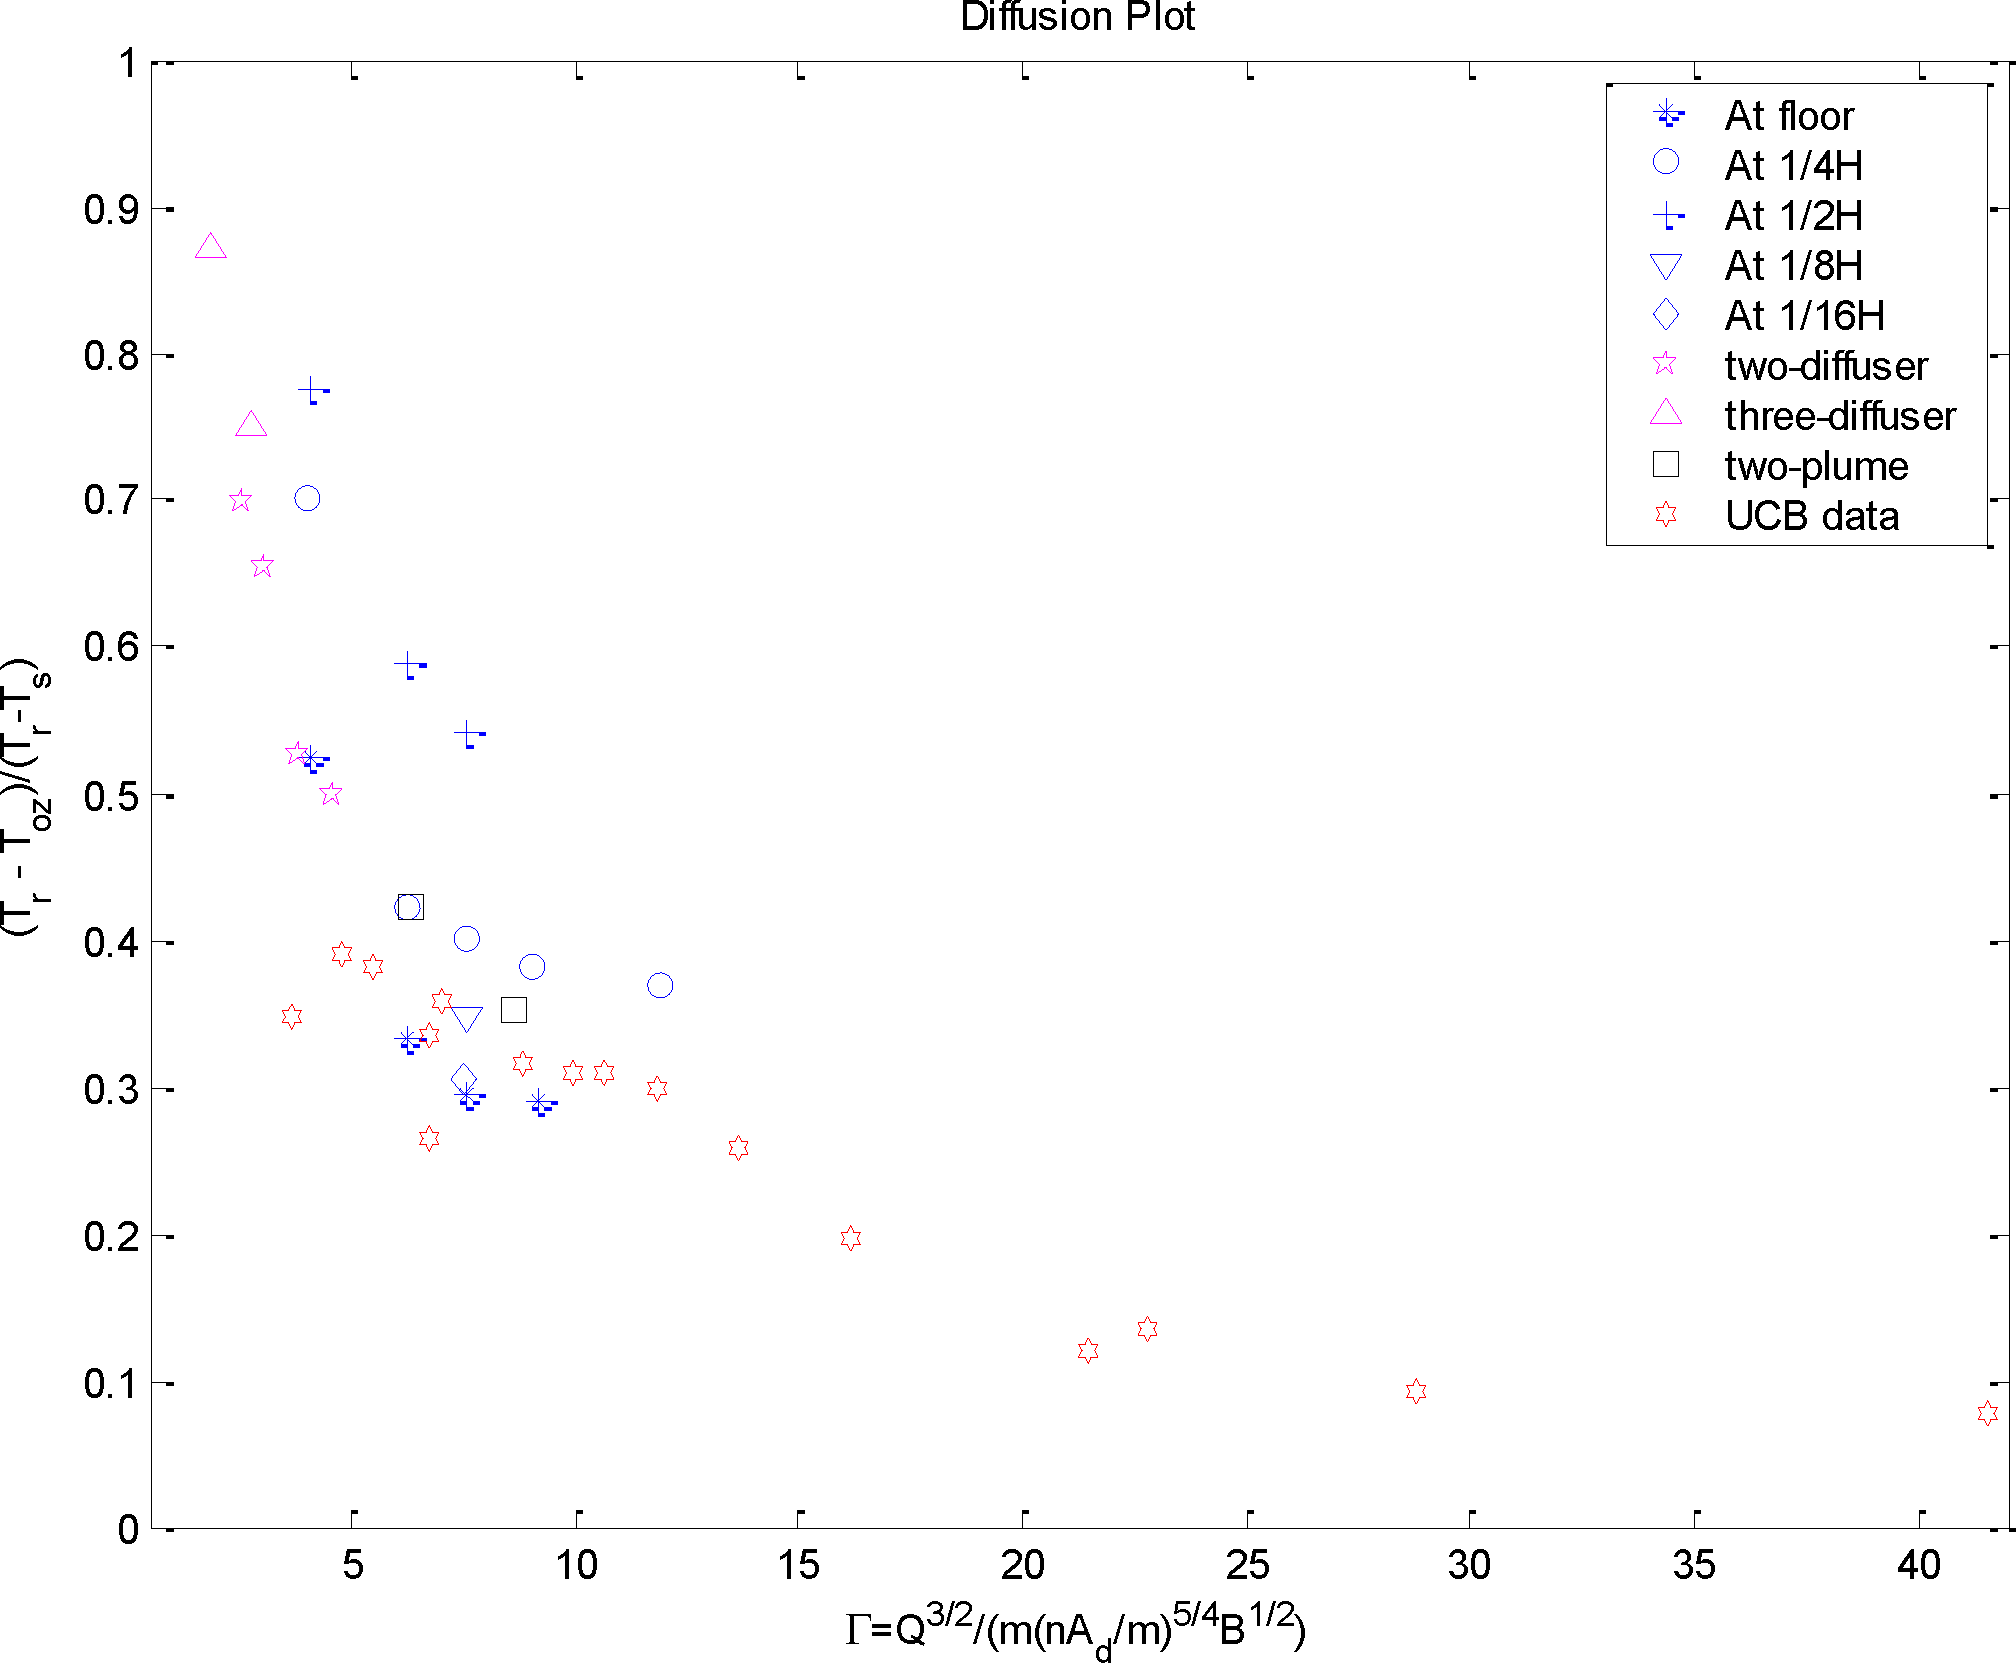
\includegraphics[width=0.9\textwidth, height=0.9\textheight, keepaspectratio=true]{media/image2469.png}
\caption{Data comparisons in the non-dimensional (a) regular \(\Gamma\)-\(\phi\) plot \protect \label{fig:data-comparisons-in-the-non-dimensional-a}}
\end{figure}

\begin{figure}[hbtp] % fig 134
\centering
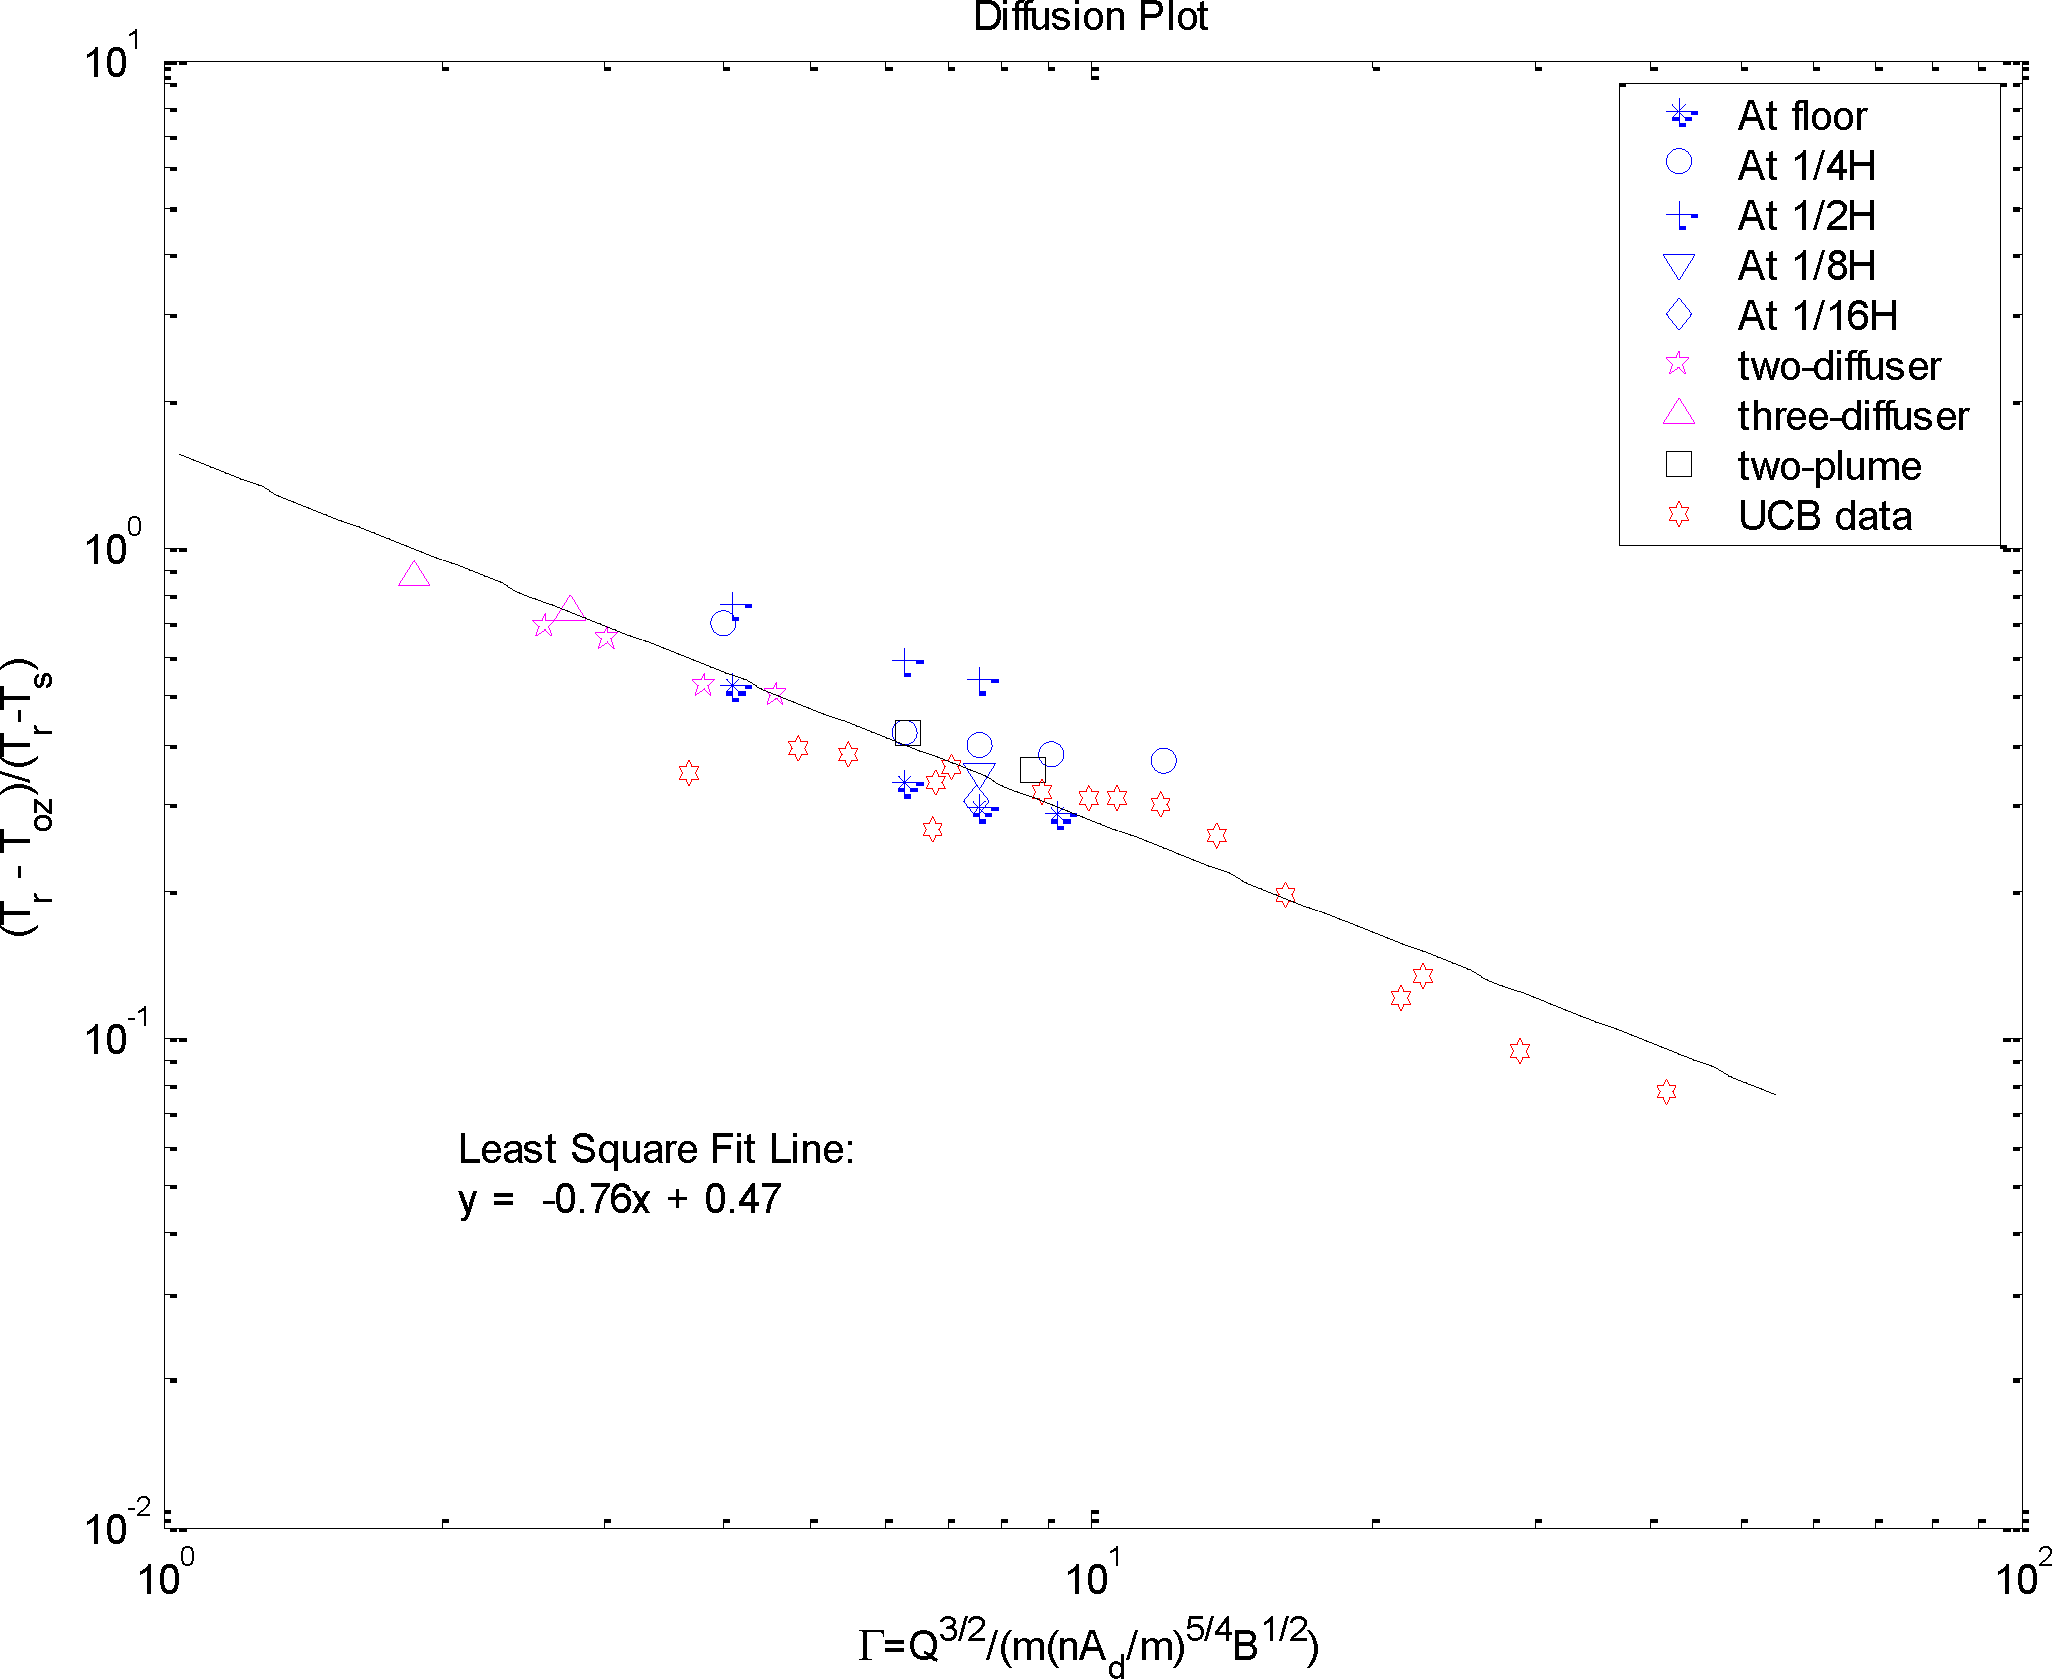
\includegraphics[width=0.9\textwidth, height=0.9\textheight, keepaspectratio=true]{media/image2470.png}
\caption{(b) log-log \(\Gamma\)-\(\phi\) plot.\} \protect \label{fig:b-log-log-g-fplot.}}
\end{figure}

The figures (Figure~\ref{fig:data-comparisons-in-the-non-dimensional-a}. Data comparisons in the non-dimensional (a) regular \(\Gamma\)-\(\phi\) plot and Figure~\ref{fig:b-log-log-g-fplot.}. (b) log-log \(\Gamma\)-\(\phi\) plot.\} show the comparisons between UCB's data and the UCSD salt tank data in the \emph{\(\Gamma\)-\(\phi\)} plot. As seen in the figures, the full-scale and small-scale data are on the same trend curve. This provides the evidence that the salt-tank experiments have included most characteristics of a UFAD system. Note that big \emph{\(\Gamma\)} (\textgreater{}20) of UCB's experiments all have large DDR (from \emph{1.19} to \emph{2.18}). The largest DDR (\emph{2.18}) even gives a negative \(({T_r} - {T_{oz}})/({T_r} - {T_s})\), which is NOT shown in the figures.)

We could work out the occupied zone temperature by using the least-square fitting line suggested in Figure~\ref{fig:b-log-log-g-fplot.}. Hence the interface height is needed to determine a entire two-layer stratification. Figure~\ref{fig:non-dimensional-interface-height-of-small} shows the dimensionless interface height\((h/\sqrt {n'A} )\) of the UCSD small-scale experiments plotted against \emph{\(\Gamma\)}. Note that for the experiments with elevated heat source, the interface heights have been modified by\(h' = h - \frac{1}{2}{h_s}\) ~where \emph{h\(_{s}\)} is the vertical position of the elevated heat source. All data then are located along a line in Figure~\ref{fig:non-dimensional-interface-height-of-small}. Since the salt-tank experiments are concluded to represent important characteristics of a full-scale UFAD room, this figure provides some guidelines for estimate the interface position in a real UFAD room.

\begin{figure}[hbtp] % fig 135
\centering
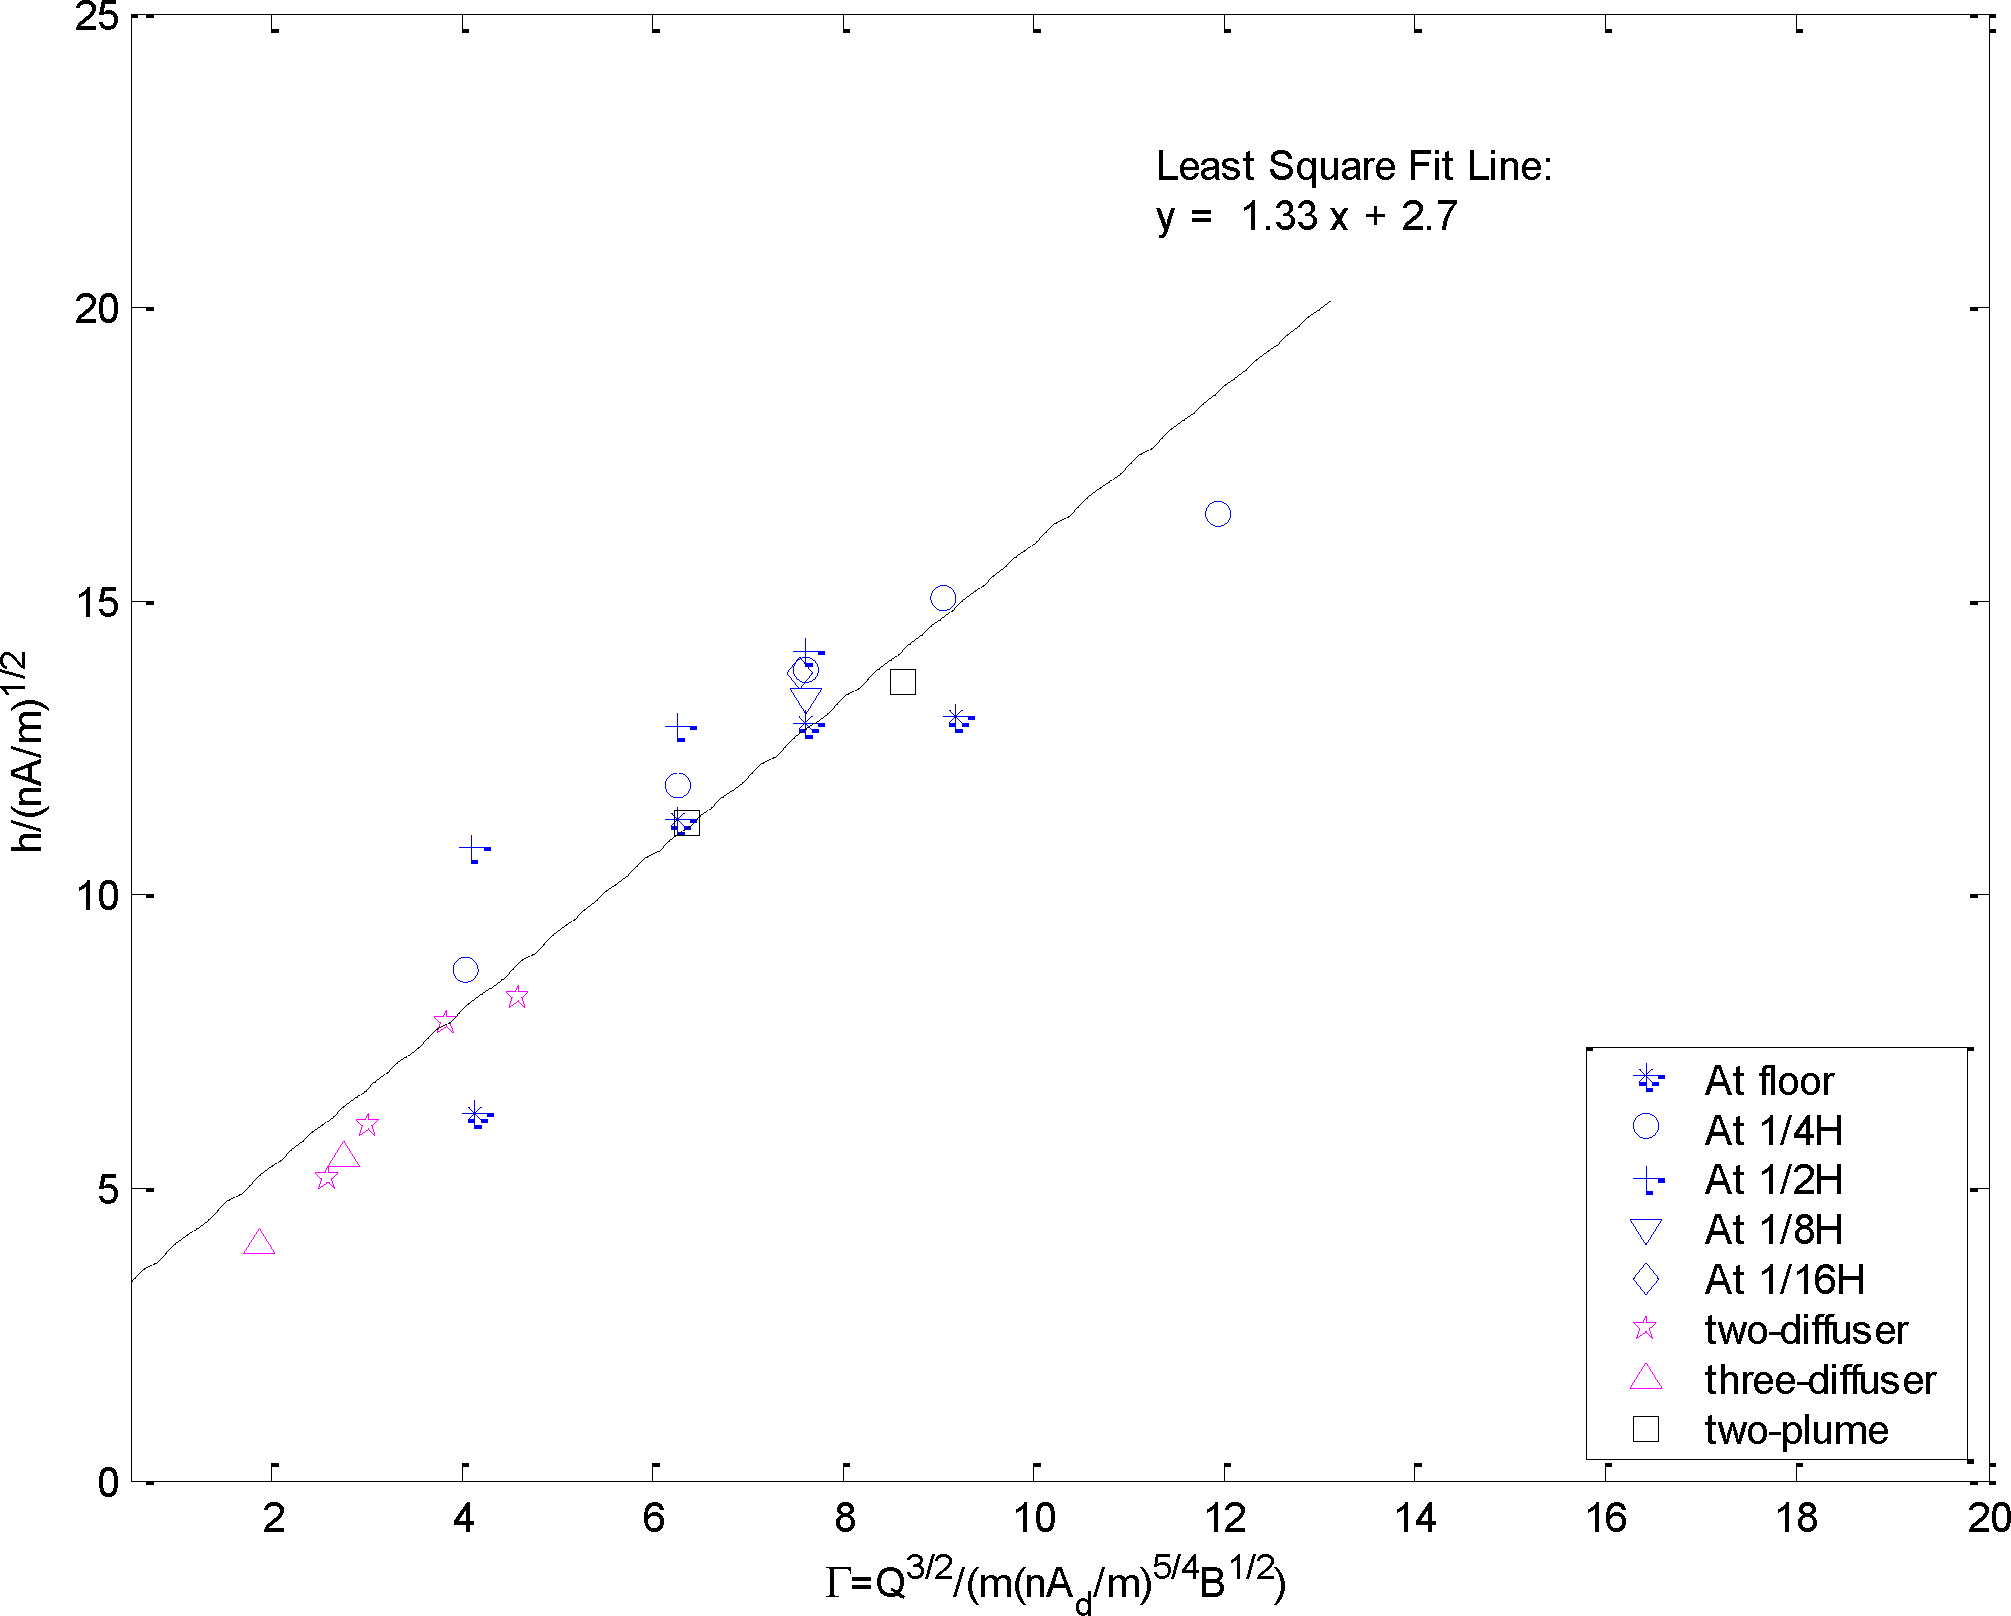
\includegraphics[width=0.9\textwidth, height=0.9\textheight, keepaspectratio=true]{media/image2474.png}
\caption{Non-dimensional interface height of small-scale experiments. \protect \label{fig:non-dimensional-interface-height-of-small}}
\end{figure}

\emph{Formulas for EnergyPlus based on the dimensionless parameter \(\Gamma\)}

If we have input including the supply temperature \emph{T\(_{s}\)} (K); the number of diffusers \emph{n}; the number of heat sources \emph{m}; the vertical position of the heat sources \emph{h\(_{s}\)} (m); the heat load \emph{W} (kW); the effective area of a diffuser \emph{A} (m\(^{2}\)); and the total supply air flow rate \emph{Q} (m\(^{3}\)/s) then the output will be;

\begin{equation}
{T_r} = \frac{{0.0281W}}{{Qg}}{T_s} + {T_s}
\end{equation}

\begin{equation}
{T_{oz}} = {T_r} - 1.6{\Gamma ^{ - 0.76}}({T_r} - {T_s})
\end{equation}

\begin{equation}
h = \sqrt {\frac{n}{m}A} (7.43ln(\Gamma ) - 1.35) + \frac{1}{2}{h_s}
\label{eq:InterfaceHeightEquation}
\end{equation}

where \emph{T\(_{r}\)} is the return temperature (K); \emph{T\(_{oz}\)} is the occupied subzone temperature (K); \emph{h} is the interface height (m); and \emph{\(\Gamma\)} is defined above.

\subsubsection{Implementation}\label{implementation-1}

The implementation closely follows the procedure described in the displacement ventilation zone model. The model predicts two temperatures that characterize the two main levels in the stratification of the room:

\begin{enumerate}
\item An occupied subzone temperature T\(_{oc}\)~representing the temperature of the occupied region;
\item An upper level temperature T\(_{mx}\) representing the temperature of the upper, mixed region and the outflow temperature.
\end{enumerate}

We will use Equation~\ref{eq:InterfaceHeightEquation} to calculate the interface height and do a heat balance calculation on each subzone. \emph{\(\Gamma\)} is given by Equation~\ref{eq:GammaFullScaleCases}. The supply air flow rate \(\dot V\) is obtained by summing all the air flows entering the zone: supply air, infiltration, ventilation, and inter-zone flow. The heat gain \(\dot Q\) is estimated by summing all the convective internal gains located in the occupied subzone -- task lights, people, equipment -- and dividing this power equally among the n plumes. With these assumptions we can describe the implementation.

The UCSD UFI model is controlled by the subroutine \emph{ManageUCSDUFModels} which is called from the \emph{RoomAirModelManager}. The \emph{RoomAirModelManager} selects which zone model will be used for each zone.

The calculation is done in subroutine \emph{CalcUCSDUI}. First we calculate the convective heat gain going into the upper and lower regions.

\begin{equation}
\begin{split}
\dot Q_{ocz} =& \dot Q_{oc,conv} + \dot Q_{tl,conv} + \dot Q_{eleq,conv} + \dot Q_{gaseq,conv} + \dot Q_{otheq,conv} + \dot Q_{hw,conv} + \dot Q_{stmeq,conv} \\
&+ \dot Q_{bb,conv} + \dot Q_{waterheater,conv} + \dot Q_{fuelcell,conv}
\end{split}
\end{equation}

\begin{equation}
{\dot Q_{mxz}} = {\dot Q_{gl,conv}} + {\dot Q_{ltp}} + {\dot Q_{htrad,conv}}
\end{equation}

\begin{equation}
{\dot Q_{tot,conv}} = {\dot Q_{ocz}} + {\dot Q_{mxz}}
\end{equation}

Next we sum up the inlet air flows in the form of MCP (mass flow rate times the air specific heat capacity) and MCPT (mass flow rate times C\(_{p}\) times air temperature).

\begin{equation}
MC{P_{zone}} = MC{P_i} + MC{P_{vent}} + MC{P_{mix}}
\end{equation}

\begin{equation}
MC{P_{sys}} = \sum\limits_{inlets} {{{\dot m}_i}} {C_{p,i}}
\end{equation}

\begin{equation}
{\dot m_{systot}} = \sum\limits_{inlets} {{{\dot m}_i}}
\end{equation}

\begin{equation}
MC{P_{tot}} = MC{P_{zone}} + MC{P_{sys}}
\end{equation}

\begin{equation}
MCP{T_{zone}} = MCP{T_i} + MCP{T_{vent}} + MCP{T_{mix}}
\end{equation}

\begin{equation}
MCP{T_{sys}} = \sum\limits_{inlets} {{{\dot m}_i}} {C_{p,i}}{T_i}
\end{equation}

\begin{equation}
MCP{T_{tot}} = MCP{T_{zone}} + MCP{T_{sys}}
\end{equation}

The number of plumes per occupant \({N_{plumesperpers}}\) ~is a user input. The total number of plumes in the zone is:

\begin{equation}
{N_{plumes}} = {N_{occ}} \cdot {N_{plumesperperson}}
\end{equation}

Using this we calculate the total power in the plumes and the power per plume.

\begin{equation}
{\dot Q_{plumes}} = {\dot Q_{ocz}}
\end{equation}

\begin{equation}
{\dot Q_{perplume}} = {\dot Q_{plumes}}/{N_{plumes}}
\end{equation}

The number of diffusers per plumes is also a user input. To obtain the number of diffusers in the zone:

\begin{equation}
{N_{diffusers}} = {N_{plumes}}\cdot {N_{diffusersperplume}}
\end{equation}

The area \emph{A\(_{diff}\)} is also a user input. For swirl diffusers and for displacement diffusers this area is used as input. For the variable area diffusers, though, we calculate the area. We assume 400 ft/min velocity at the diffuser and a design flow rate per diffuser is 150 cfm (.0708 m\(^{3}\)/s). The design area of the diffuser is 150 ft\(^{3}\)/min / 400 ft/min = .575 ft\(^{2}\) = .035 m\(^{2}\). Then the variable area each time step is

\begin{equation}
{A_{diff}} = {\dot m_{systot}}/(.0708\cdot {N_{diffusers}})
\end{equation}

We now calculate the height fraction \emph{Fr\(_{hb}\)} (height of boundary layer divided by the total zone height).

\begin{equation}
\Gamma  = \frac{{{{({{\dot m}_{systot}}\cdot \cos ({\theta_{throw}}))}^{3/2}}}}{{{N_{plumes}}{{({N_{diffusersperplume}}\cdot {A_{diff}})}^{5/4}}{{(0.0281\cdot 0.001\cdot {{\dot Q}_{plumes}})}^{1/2}}}}
\end{equation}

\begin{equation}
F{r_{hb}} = \frac{{{{({N_{diffusersperplume}}\cdot {A_{diff}})}^{1/2}}(7.43\ln (\Gamma ) - 1.35 + 0.5{H_s})}}{{{H_{ceil}}}}
\end{equation}

where \emph{\(\theta_{throw}\)} is a user input: the angle between the diffuser slots and vertical; and \emph{H\(_{s}\)} is the source height above the floor (m).

Next we iterate over the following 2 steps.

\subsubsection{Iterative procedure}\label{iterative-procedure-1}

\begin{enumerate}
\item Call subroutine \emph{HcUCSDUF} to calculate a convective heat transfer coefficient for each surface in the zone, an effective air temperature for each surface, and HA\(_{mx}\), HAT\(_{mx}\), HA\(_{oc}\), HAT\(_{oc}\). Here HA is \(\sum\limits_{surfaces} {{h_{c,i}} \cdot {A_i}}\) for a region and HAT is \(\sum\limits_{surfaces} {{h_{c,i}} \cdot {A_i}} \cdot {T_i}\) for a region. The sum is over all the surfaces bounding the region; \({{h_{c,i}}}\) is the convective heat transfer coefficient for surface i, \({A_i}\) is the area of surface i, and \({T_i}\) is the surface temperature of surface i.
\item Calculate the two subzone temperatures: \emph{T\(_{oc}\)} and \emph{T\(_{mx}\)}.
\end{enumerate}

The h\(_{c}\)'s calculated in step 1 depend on the subzone temperatures. In turn the subzone temperatures depend on the HA and HAT's calculated in step 1. Hence the need for iteration.

Next we describe Steps 1 and 2 in more detail.

\subsubsection{Step 1}\label{step-1-1}

Subroutine \emph{HcUCSDUF} is quite straightforward. It loops through all the surfaces in each zone and decides whether the surface is located in the upper, mixed subzone or the lower, occupied subzone, or if the surface is in both subzones. If entirely in one subzone the subzone temperature is stored in the surface effective temperature variable \emph{SurfTempEffBulkAir(SurfNum)} and h\(_{c}\) for the surface is calculated by a call to subroutine \emph{CalcDetailedHcInForDVModel}. This routine uses the ``detailed'' natural convection coefficient calculation that depends on surface tilt and \(\Delta {T^{1/3}}\) . This calculation is appropriate for situations with low air velocity.

For surfaces that bound 2 subzones, the subroutine calculates h\(_{c}\) for each subzone and then averages them, weighting by the amount of surface in each subzone.

During the surface loop, once the h\(_{c}\)~for a surface is calculated, the appropriate subzone HA and HAT sums are incremented. If a surface is in 2 subzones the HA and HAT for each subzone are incremented based on the area of the surface in each subzone.

\subsubsection{Step 2}\label{step-2}

The calculation of~ subzone temperatures follows the method used in the \textbf{\emph{ZoneTempPredictorCorrector}} module and described in the section \textbf{Basis for the System and Zone Integration}. Namely a third order finite difference expansion of the temperature time derivative is used in updating the subzone temperatures. Otherwise the subzone temperatures are obtained straightforwardly by solving an energy balance equation for each subzone.

\begin{equation}
  \begin{array}{cl}
    T_{oc} & = \frac{(C_{air,oc} \cdot (3 \cdot T_{ - 1,oc} - (3/2) \cdot T_{ - 2,oc} + (1/3) \cdot T_{ - 3,oc}) + \dot Q_{ocz} \cdot Fr_{gains} + HAT_{oc} + MCPT_{tot})} {((11/6) \cdot C_{air,oc} + HA_{oc} + MCP_{tot})} \\
    T_{mx} & = \frac{(C_{air,mx} \cdot (3 \cdot T_{ - 1,mx} - (3/2) \cdot T_{ - 2,mx} + (1/3) \cdot T_{ - 3,mx}) + \dot Q_{ocz} \cdot (1 - Fr_{gains}) + \dot Q_{mxz} + HAT_{mx} + T_{oc} \cdot MCP_{tot})} {((11/6) \cdot C_{air,mx} + HA_{mx} + MCP_{tot})}
  \end{array}
\end{equation}

Here \({C_{air,oc}}\) and \({C_{air,mx}}\) are the heat capacities of the air volume in each subzone. \({C_{air,mx}}\) is calculated by:

\begin{equation}
{R_{air,mx}} = {V_{mx}} \cdot \left( {\Delta {z_{mx}}/{z_{ceil}}} \right) \cdot {\rho_{air,mx}} \cdot {c_{p,air,mx}} \cdot Mu{l_{cap}}/\left( {\Delta {t_z} \cdot 3600} \right)
\end{equation}

\begin{equation}
{c_{air,mx}} = {R_{air,mx}} \cdot \Delta {t_z}/\Delta {t_{sys}}
\end{equation}

The gains fraction \(F{r_{gains}}\) is a user input via a schedule. It is the fraction of the convective gains in the occupied subzone that remain in that subzone.

The other subzone air heat capacities are calculated in the same manner.

\subsubsection{Mixed calculation}\label{mixed-calculation-1}

The above iterative procedure assumed that the UFAD nonuniform zone model was appropriate: i.e., conditions were favorable temperature stratification in the zone. Now that this calculation is complete and the subzone temperatures and depths calculated, we check to see if this assumption was justified. If not, zone conditions must be recalculated assuming a well-mixed zone.

If \({T_{mx}} < {T_{oc}}\) or \(MC{P_{tot}} \le 0\) or \({H_{fr}} \cdot {H_{ceil}} < \Delta {z_{occ,\min }}\), then the following mixed calculation will replace the UFAD interior zone calculation.

\textbf{Note:} \(\Delta {z_{occ,min}}\) is the minimum thickness of occupied subzone. It is set to 0.2 meters.

The mixed calculation iteratively calculates surface convection coefficients and room temperature just like the displacement ventilation calculation described above. In the mixed case however, only one zone temperature \emph{T\(_{avg}\)} is calculated. The 3 subzone temperatures are then set equal to \emph{T\(_{avg}\)}.

First, \emph{Fr\(_{hb}\)}~ is set equal to zero.

Then the code iterates over these steps.

Calculate \emph{T\(_{avg}\)} using:

\begin{equation}
  \begin{array}{rl}
    T_{avg} &= ({C_{air,z}} \cdot (3 \cdot {T_{ - 1,z}} - (3/2) \cdot {T_{ - 2,z}} + (1/3) \cdot {T_{ - 3,z}}) \\
            &+ {{\dot Q}_{tot,conv}} + HA{T_{oc}} + HA{T_{mx}} + MCP{T_{tot}})/((11/6) \cdot {C_{air,z}} + H{A_{oc}} + H{A_{mx}} + MC{P_{tot}})
  \end{array}
\end{equation}

\begin{equation}
{T_{mx}} = {T_{avg}}
\end{equation}

\begin{equation}
{T_{oc}} = {T_{avg}}
\end{equation}

Call \emph{HcUCSDUF} to calculate the \emph{h\(_{c}\)}'s.

Repeat step 1

\subsubsection{Final calculations}\label{final-calculations-1}

The UFAD interior zone calculation finishes by calculating some report variables.

We define heights:

\begin{equation}
{H_{trans}} = F{r_{hb}} \cdot {H_{ceil}}
\end{equation}

\begin{equation}
{H_{mxavg}} = \left( {{H_{ceil}} + {H_{trans}}} \right)/2
\end{equation}

\begin{equation}
{H_{ocavg}} = {H_{trans}}/2
\end{equation}

Using the user defined comfort height we calculate the comfort temperature.

If mixing:

\begin{equation}
{T_{comf}} = {T_{avg}}
\end{equation}

If UFAD:

If \({H_{comf}} < {H_{ocavg}}\):

\begin{equation}
{T_{comf}} = {T_{occ}}
\end{equation}

Else if \({H_{comf}} \ge {H_{ocavg}}\) ~and \({H_{comf}} < {H_{mxavg}}\):

\begin{equation}
{T_{comf}} = \left( {{T_{oc}}\left( {{H_{mxavg}} - {H_{comf}}} \right) + {T_{mx}}\left( {{H_{comf}} - {H_{ocavg}}} \right)} \right)/\left( {{H_{mxavg}} - {H_{ocavg}}} \right)
\end{equation}

Else if \({H_{comf}} \ge {H_{mxavg}}\) ~and \({H_{comf}} < {H_{ceil}}\):

\begin{equation}
{T_{comf}} < {T_{mx}}
\end{equation}

Using the user defined thermostat height we calculate the temperature at the thermostat.

If mixing:

\begin{equation}
{T_{stat}} < {T_{avg}}
\end{equation}

If UFAD:

If\({H_{stat}} < {H_{ocavg}}\):

\begin{equation}
{T_{stat}} = {T_{occ}}
\end{equation}

Else if \({H_{stat}} \ge {H_{ocavg}}\) ~and \({H_{stat}} < {H_{mxavg}}\):

\begin{equation}
{T_{stat}} = \left( {{T_{oc}}\left( {{H_{mxavg}} - {H_{stat}}} \right) + {T_{mx}}\left( {{H_{stat}} - {H_{ocavg}}} \right)} \right)/\left( {{H_{mxavg}} - {H_{ocavg}}} \right)
\end{equation}

Else if \({H_{stat}} \ge {H_{mxavg}}\) ~and \({H_{stat}} < {H_{ceil}}\):

\begin{equation}
{T_{stat}} = {T_{mx}}
\end{equation}

The average temperature gradient is:

If \({H_{mxavg}} - {H_{occavg}} > 0.1\):

\begin{equation}
Grad{T_{avg}} = ({T_{mx}} - {T_{occ}})/({H_{mxavg}} - {H_{occavg}})
\end{equation}

else \(Grad{T_{avg}} = 0.0\).

Finally, the zone node temperature is set to \emph{T\(_{mx}\)}.

Other variables that are reported out are \(\Gamma\) and \(\phi\).

\begin{equation}
\phi  = ({T_{mx}} - {T_{occ}})/({T_{mx}} - {T_{sup}})
\end{equation}

where \({T_{sup}}\) is the zone supply air temperature.

\subsection{Under-Floor Air Distribution Exterior Zone Model}\label{under-floor-air-distribution-exterior-zone-model}

\subsubsection{Overview}\label{overview-2-001}

The input object RoomAirSettings:UnderFloorAirDistributionExterior provides a simple model for heat transfer and a nonuniform vertical temperature profile for exterior zones of a UFAD system. These zones are expected to be dominated by internal loads, a portion of which (such as occupants and workstations) will act to generate plumes, and by window solar and conduction heat gains. The solar radiation penetrating the room is not expected to generate plumes. However, a window plume is likely to be generated in sunny conditions, particularly if an interior blind is deployed. Thus the exterior UFAD zone will have potentially have plumes from people and equipment and plumes arising from the windows. The plumes act to potentially create room air stratification, depending on the type \& number of diffusers, the amount and type of load, and the system flowrate. In order to better model this situation the fully-mixed room air approximation that is currently used in most whole building analysis tools is extended to a two node approach, with the purpose of obtaining a first order precision model for vertical temperature profiles for the exterior zones of UFAD systems. The use of 2 nodes allows for greatly improved prediction of thermal comfort and overall building energy performance for the increasingly popular UFAD systems.

TheUCSD UFAD Exterior Zone Model is one of the non-uniform zone models provided through the Room Air Manager in EnergyPlus. The intent is to provide a selection of useful non-uniform zone air models to enable the evaluation of air-conditioning techniques that use stratified or partially stratified room air. Such techniques include displacement ventilation (DV) and underfloor air distribution (UFAD) systems. The methodology can also include natural displacement ventilation and also wind-driven cross-ventilation (CV).

\subsubsection{Underfloor air distribution systems}\label{underfloor-air-distribution-systems-1}

UFAD systems represent, in terms of room air stratification, an intermediate condition between a well-mixed zone and displacement ventilation. Air is supplied through an underfloor plenum at low pressure through diffusers in the raised floor. The diffusers can be of various types: e.g., swirl, variable-area, displacement, and produce more or less mixing in the zone. UFAD systems are promoted as saving energy due to: higher supply air temperature; low static pressure; cooler conditions in the occupied subzone than in the upper subzone; and sweeping of some portion of the convective load (from ceiling lights, for instance) into the return air without interaction with the occupied region of the zone.

Modeling a UFAD system is quite complex and involves considerably more than just a non-uniform zone model. The zones' coupling to the supply and return plenums must be modeled accurately (particularly radiative transfer from a warm ceiling to a cool floor and on into the supply plenum by conduction). The supply plenum must be accurately modeled, giving a good estimate of the supply air temperature and conduction heat transfer between supply \& return plenums through the slab. The HVAC system must be modeled including return air bypass and various types of fan powered terminal units.

The UCSD UFAD exterior zone model is similar to the UCSD interior zone model. The most obvious difference is that the exterior UFAD has 2 different types of plume sources: people \& equipment and windows. Like the UCSD UFAD interior model it is a plume equation based multi-layer model (2 layers in this case). The zone is modeled as being divided into 2 well separated subzones which we denote as ``occupied'' and ``upper''. Each subzone is treated as having a single temperature. The boundary between the 2 subzones moves up \& down each time step as a function of zone loads and supply air flow rate. Thus at each HVAC time step, the height of the boundary above the floor must be calculated, portions of surfaces assigned to each subzone, and a separate convective heat balance performed on each subzone.

\subsubsection{Model Description}\label{model-description-2-001}

As in the interior zone case, we define 2 dimensionless parameters: \(\Gamma\) and \(\phi\). The definitions of the 2 parameters are the same as in the previous section (Equations~\ref{eq:GammaSinglePlumeSingleDiffuser},~\ref{eq:GammaMultiDiffuserMultiSource},~\ref{eq:GammaFullScaleCases},~\ref{eq:PhiSmallScaleCases}, and~\ref{eq:PhiFullScaleCases}). As in the previous case, the experimental data can be plotted versus \(\Gamma\) and lines fitted to the data give the following formulas for occupied subzone temperature and interface height.

\begin{equation}
{T_{oz}} = {T_r} - 1.4{\Gamma ^{ - 0.6}}({T_r} - {T_s})
\end{equation}

\begin{equation}
h = \sqrt {\frac{n}{m}A} (11.03ln(\Gamma ) - 10.73) + \frac{1}{2}{h_s}
\label{eq:InterfaceHeightUFAD}
\end{equation}

where \emph{T\(_{oz}\)} is the occupied subzone temperature (K); \emph{T\(_{r}\)}~is the return temperature (K); \emph{\(\Gamma\)}~is the dimensionless height parameter defined above; \emph{T\(_{s}\)} is the supply temperature (K); \emph{h} is the interface height (m); \emph{n} is the number of diffusers; \emph{m} is the number of heat sources; \emph{A} is the effective area of a diffuser (m\(^{2}\)); and \emph{h\(_{s}\)} is the vertical position of the heat sources (m). The formula for \emph{T\(_{r}\)} is the same as in the previous section.

\subsubsection{Implementation}\label{implementation-2}

The implementation closely follows the procedure described in the UFAD interior zone model. The model predicts two temperatures that characterize the two main levels in the stratification of the room:

\begin{enumerate}
\item An occupied subzone temperature T\(_{oc}\)~representing the temperature of the occupied region;
\item An upper level temperature T\(_{mx}\) representing the temperature of the upper, mixed region and the outflow temperature.
\end{enumerate}

We will use Equation~\ref{eq:InterfaceHeightUFAD} to calculate the interface height and do a heat balance calculation on each subzone. \emph{\(\Gamma\)} is given by Equation~\ref{eq:GammaFullScaleCases}. The supply air flow rate \(\dot V\) is obtained by summing all the air flows entering the zone: supply air, infiltration, ventilation, and inter-zone flow. The heat gain \(\dot Q\) is estimated by summing all the convective internal gains located in the occupied subzone -- task lights, people, equipment -- and adding to this the convective gain coming from the window surface. With these assumptions we can describe the implementation.

The UCSD UFE model is controlled by the subroutine \emph{ManageUCSDUFModels} which is called from the \emph{RoomAirModelManager}. The \emph{RoomAirModelManager} selects which zone model will be used for each zone.

The calculation is done in subroutine \emph{CalcUCSDUEI}. First we calculate the convective heat gain going into the upper and lower regions.

\begin{equation}
\begin{split}
\dot Q_{ocz} =& \dot Q_{oc,conv} + \dot Q_{tl,conv} + \dot Q_{eleq,conv} + \dot Q_{gaseq,conv} + \dot Q_{otheq,conv} + \dot Q_{hw,conv} + \dot Q_{stmeq,conv} \\
&+ \dot Q_{bb,conv} + \dot Q_{waterheater,conv} + \dot Q_{fuelcell,conv}
\end{split}
\end{equation}

\begin{equation}
{\dot Q_{mxz}} = {\dot Q_{gl,conv}} + {\dot Q_{ltp}} + {\dot Q_{htrad,conv}}
\end{equation}

\begin{equation}
{\dot Q_{tot,conv}} = {\dot Q_{ocz}} + {\dot Q_{mxz}}
\end{equation}

Next we sum up the inlet air flows in the form of MCP (mass flow rate times the air specific heat capacity) and MCPT (mass flow rate times C\(_{p}\) times air temperature).

\begin{equation}
MC{P_{zone}} = MC{P_i} + MC{P_{vent}} + MC{P_{mix}}
\end{equation}

\begin{equation}
MCP_{sys} = \sum\limits_{inlets} {\dot m_i C_{p,i}}
\end{equation}

\begin{equation}
{\dot m_{systot}} = \sum\limits_{inlets} {{{\dot m}_i}}
\end{equation}

\begin{equation}
MC{P_{tot}} = MC{P_{zone}} + MC{P_{sys}}
\end{equation}

\begin{equation}
MCP{T_{zone}} = MCP{T_i} + MCP{T_{vent}} + MCP{T_{mix}}
\end{equation}

\begin{equation}
MCP{T_{sys}} = \sum\limits_{inlets} {{{\dot m}_i}} {C_{p,i}}{T_i}
\end{equation}

\begin{equation}
MCP{T_{tot}} = MCP{T_{zone}} + MCP{T_{sys}}
\end{equation}

For exterior zone model, we assume one plume: \({N_{plumes}} = 1\). The number of diffusers in the zone \({N_{diffusers}}\) is a user input.

The area \emph{A\(_{diff}\)} is also a user input. For swirl diffusers, linear bar grilles, and displacement diffusers this area is used as input. For the variable area diffusers, though, we calculate the area. We assume 400 ft/min velocity at the diffuser and a design flow rate per diffuser is 150 cfm (.0708 m\(^{3}\)/s). The design area of the diffuser is 150 ft\(^{3}\)/min / 400 ft/min = .575 ft\(^{2}\) = .035 m\(^{2}\). Then the variable area each time step is:

\begin{equation}
{A_{diff}} = {\dot m_{systot}}/(.0708\cdot {N_{diffusers}})
\end{equation}

We now make an initial estimate of the convective gain from the windows.

\begin{equation}
{\dot Q_{win,conv}} = \sum\limits_{i = 1,{n_{win}}} {{h_{c,i}}} {A_{win,i}}{T_{winsurf,i}} - {h_{c,i}}{A_{win,i}}{T_{mat}}
\end{equation}

Then:

\begin{equation}
{\dot Q_{plumes}} = {\dot Q_{ocz}} + {\dot Q_{win,conv}}
\end{equation}

We now calculate the height fraction \emph{Fr\(_{hb}\)} (height of boundary layer divided by the total zone height).

\begin{equation}
\Gamma  = \frac{{{{({{\dot m}_{systot}}\cdot \cos ({\theta_{throw}}))}^{3/2}}}}{{{{({N_{diffusers}}\cdot {A_{diff}})}^{5/4}}{{(0.0281\cdot 0.001\cdot {{\dot Q}_{plumes}})}^{1/2}}}}
\end{equation}

\begin{equation}
F{r_{hb}} = \frac{{{{({N_{diffusers}}\cdot {A_{diff}})}^{1/2}}(11.03ln(\Gamma ) - 10.73 + 0.5{H_s})}}{{{H_{ceil}}}}
\end{equation}

where \emph{\(\theta_{throw}\)} is a user input: the angle between the diffuser slots and vertical; and \emph{H\(_{s}\)} is the source height above the floor (m).

Next we iterate over the following 2 steps.

\subsubsection{Iterative procedure}\label{iterative-procedure-2}

\begin{enumerate}
\item Call subroutine \emph{HcUCSDUF} to calculate a convective heat transfer coefficient for each surface in the zone, an effective air temperature for each surface, and HA\(_{mx}\), HAT\(_{mx}\), HA\(_{oc}\), HAT\(_{oc}\), HA\(_{mx,win}\), HAT\(_{mx,win}\), HA\(_{oc,win}\),and HAT\(_{oc,win}\). Here HA is \(\sum\limits_{surfaces} {{h_{c,i}} \cdot {A_i}}\) for a region and HAT is \(\sum\limits_{surfaces} {{h_{c,i}} \cdot {A_i}} \cdot {T_i}\) for a region. The sum is over all the surfaces bounding the region; \({h_{c,i}}\) is the convective heat transfer coefficient for surface i, \({A_i}\) is the area of surface i, and \({T_i}\) is the surface temperature of surface i. Variables with the \emph{win} subscript are summed over window surfaces only. Then the convective gain from the window is recalculated using Equation~\ref{eq:QdotwinconvUSCDUFAD} and the power in the plume is recalculated: \({\dot Q_{plumes}} = {\dot Q_{ocz}} + {\dot Q_{win,conv}}\) .
\item Calculate the two subzone temperatures: \emph{T\(_{oc}\)} and \emph{T\(_{mx}\)}.
\end{enumerate}

\begin{equation}
{\dot Q_{win,conv}} = HA{T_{mx,win}} + HA{T_{oc,win}} - H{A_{mx,win}}{T_{mx}} - H{A_{oc,win}}{T_{oc}}
\label{eq:QdotwinconvUSCDUFAD}
\end{equation}

The h\(_{c}\)'s calculated in step 1 depend on the subzone temperatures. In turn the subzone temperatures depend on the HA and HAT's calculated in step 1. Hence the need for iteration.

Next we describe Steps 1 and 3 in more detail.

\subsubsection{Step 1}\label{step-1-2}

Subroutine \emph{HcUCSDUF} is quite straightforward. It loops through all the surfaces in each zone and decides whether the surface is located in the upper, mixed subzone or the lower, occupied subzone, or if the surface is in both subzones. If entirely in one subzone the subzone temperature is stored in the surface effective temperature variable \emph{SurfTempEffBulkAir(SurfNum)} and h\(_{c}\) for the surface is calculated by a call to subroutine \emph{CalcDetailedHcInForDVModel}. This routine uses the ``detailed'' natural convection coefficient calculation that depends on surface tilt and \(\Delta {T^{1/3}}\) . This calculation is appropriate for situations with low air velocity.

For surfaces that bound 2 subzones, the subroutine calculates h\(_{c}\) for each subzone and then averages them, weighting by the amount of surface in each subzone.

During the surface loop, once the h\(_{c}\)~for a surface is calculated, the appropriate subzone HA and HAT sums are incremented. If a surface is in 2 subzones the HA and HAT for each subzone are incremented based on the area of the surface in each subzone. The subroutine calculates a separate HA and HAT for the windows for use in calculating the window convective gain.

\subsubsection{Step 2}\label{step-2-1}

The calculation of~ subzone temperatures follows the method used in the \textbf{\emph{ZoneTempPredictorCorrector}} module and described in the section \textbf{Basis for the System and Zone Integration}. Namely a third order finite difference expansion of the temperature time derivative is used in updating the subzone temperatures. Otherwise the subzone temperatures are obtained straightforwardly by solving an energy balance equation for each subzone.

\begin{equation}
  \begin{array}{cl}
    T_{oc} & = \frac{(C_{air,oc} \cdot (3 \cdot T_{ - 1,oc} - (3/2) \cdot T_{ - 2,oc} + (1/3) \cdot T_{ - 3,oc}) + \dot Q_{ocz} \cdot Fr_{gains} + HAT_{oc} + MCPT_{tot})} {((11/6) \cdot C_{air,oc} + HA_{oc} + MCP_{tot})} \\
    T_{mx} & = \frac{(C_{air,mx} \cdot (3 \cdot T_{ - 1,mx} - (3/2) \cdot T_{ - 2,mx} + (1/3) \cdot T_{ - 3,mx}) + \dot Q_{ocz} \cdot (1 - Fr_{gains}) + \dot Q_{mxz} + HAT_{mx} + T_{oc} \cdot MCP_{tot})} {((11/6) \cdot C_{air,mx} + HA_{mx} + MCP_{tot})}
  \end{array}
\end{equation}

Here \({C_{air,oc}}\) and \({C_{air,mx}}\) are the heat capacities of the air volume in each subzone. \({C_{air,mx}}\) is calculated by:

\begin{equation}
{R_{air,mx}} = {V_{mx}} \cdot \left( {\Delta {z_{mx}}/{z_{ceil}}} \right) \cdot {\rho_{air,mx}} \cdot {c_{p,air,mx}} \cdot Mu{l_{cap}}/\left( {\Delta {t_z} \cdot 3600} \right)
\end{equation}

\begin{equation}
{c_{air,mx}} = {R_{air,mx}} \cdot \Delta {t_z}/\Delta {t_{sys}}
\end{equation}

The gains fraction \(F{r_{gains}}\) is a user input via a schedule. It is the fraction of the convective gains in the occupied subzone that remain in that subzone.

The other subzone air heat capacities are calculated in the same manner.

\subsubsection{Mixed calculation}\label{mixed-calculation-2}

The above iterative procedure assumed that the UFAD zone model was applicable: i.e., conditions were favorable temperature stratification in the zone. Now that this calculation is complete and the subzone temperatures and depths calculated, we check to see if this assumption was justified. If not, zone conditions must be recalculated assuming a well-mixed zone.

If \({T_{mx}} < {T_{oc}}\) or \(MC{P_{tot}} \le 0\) or \({H_{fr}} \cdot {H_{ceil}} < \Delta {z_{occ,\min }}\), then the following mixed calculation will replace the UFAD exterior zone calculation.

\textbf{Note:} \(\Delta {z_{occ,min}}\) is the minimum thickness of occupied subzone. It is set to 0.2 meters.

The mixed calculation iteratively calculates surface convection coefficients and room temperature just like the displacement ventilation calculation described above. In the mixed case however, only one zone temperature \emph{T\(_{avg}\)} is calculated. The 2 subzone temperatures are then set equal to \emph{T\(_{avg}\)}.

First, \emph{Fr\(_{hb}\)} is set equal to zero.

Then the code iterates over these steps.

Calculate \emph{T\(_{avg}\)} using:

\begin{equation}
  \begin{array}{rl}
    T_{avg} &= ({C_{air,z}} \cdot (3 \cdot {T_{ - 1,z}} - (3/2) \cdot {T_{ - 2,z}} + (1/3) \cdot {T_{ - 3,z}}) \\
            &+ {{\dot Q}_{tot,conv}} + HA{T_{oc}} + HA{T_{mx}}MCP{T_{tot}})/((11/6) \cdot {C_{air,z}} + H{A_{oc}} + H{A_{mx}} + MC{P_{tot}})
  \end{array}
\end{equation}

\begin{equation}
{T_{mx}} = {T_{avg}}
\end{equation}

\begin{equation}
{T_{oc}} = {T_{avg}}
\end{equation}

Call \emph{HcUCSDUF} to calculate the \emph{h\(_{c}\)}'s.

Repeat step 1.

\subsubsection{Final calculations}\label{final-calculations-2}

The UFAD exterior zone calculation finishes by calculating some report variables.

We define heights:

\begin{equation}
{H_{trans}} = F{r_{hb}} \cdot {H_{ceil}}
\end{equation}

\begin{equation}
{H_{mxavg}} = \left( {{H_{ceil}} + {H_{trans}}} \right)/2
\end{equation}

\begin{equation}
{H_{ocavg}} = {H_{trans}}/2
\end{equation}

Using the user defined comfort height we calculate the comfort temperature.

If mixing:

\begin{equation}
{T_{comf}} = {T_{avg}}
\end{equation}

If UFAD:

If~ \({H_{comf}} < {H_{ocavg}}\):

\begin{equation}
{T_{comf}} = {T_{occ}}
\end{equation}

Else if \({H_{comf}} \ge {H_{ocavg}}\) ~and \({H_{comf}} < {H_{mxavg}}\):

\begin{equation}
{T_{comf}} = \left( {{T_{oc}}\left( {{H_{mxavg}} - {H_{comf}}} \right) + {T_{mx}}\left( {{H_{comf}} - {H_{ocavg}}} \right)} \right)/\left( {{H_{mxavg}} - {H_{ocavg}}} \right)
\end{equation}

Else if \({H_{comf}} \ge {H_{mxavg}}\) ~and \({H_{comf}} < {H_{ceil}}\):

\begin{equation}
{T_{comf}} < {T_{mx}}
\end{equation}

Using the user defined thermostat height, we calculate the temperature at the thermostat.

If mixing:

\begin{equation}
{T_{stat}} = {T_{avg}}
\end{equation}

If UFAD:

If\({H_{stat}} < {H_{ocavg}}\):

\begin{equation}
{T_{stat}} = {T_{occ}}
\end{equation}

Else if \({H_{stat}} \ge {H_{ocavg}}\) ~and \({H_{stat}} < {H_{mcavg}}\):

\begin{equation}
{T_{stat}} = \left( {{T_{oc}}\left( {{H_{mxavg}} - {H_{stat}}} \right) + {T_{mx}}\left( {{H_{stat}} - {H_{ocavg}}} \right)} \right)/\left( {{H_{mxavg}} - {H_{ocavg}}} \right)
\end{equation}

Else if \({H_{stat}} \ge {H_{mxavg}}\) ~and \({H_{stat}} < {H_{ceil}}\):

\begin{equation}
{T_{stat}} = {T_{mx}}
\end{equation}

The average temperature gradient is:

If \({H_{mxavg}} - {H_{occavg}} > 0.1\):

\begin{equation}
Grad{T_{avg}} = ({T_{mx}} - {T_{occ}})/({H_{mxavg}} - {H_{occavg}})
\end{equation}

else \(Grad{T_{avg}} = 0.0\).

Finally, the zone node temperature is set to \emph{T\(_{mx}\)}.

Other variables that are reported out are \(\Gamma\) and \(\phi\).

\begin{equation}
\phi  = ({T_{mx}} - {T_{occ}})/({T_{mx}} - {T_{sup}})
\end{equation}

where \({T_{sup}}\) is the zone supply air temperature.

\subsection{Cross Ventilation Room Air Model}\label{cross-ventilation-room-air-model}

\subsubsection{Overview}\label{overview-3-001}

The input object RoomAirSettings:CrossVentilation provides a simple model, developed by UCSD, for heat transfer and vertical temperature profile prediction in cross ventilated rooms. This model was developed using scaling analysis, experimental correlations, computational fluid dynamics, and approximate solutions of the Navier-Stokes equations. The model distinguishes two regions in the room, the main jet region and the recirculations, and predicts characteristic airflow velocities and average air temperatures. The model consists of a set of analytical expressions that clearly display the first order effects of room geometry and inflow characteristics on Cross Ventilation airflow and heat transfer.

\subsubsection{Cross-Ventilation}\label{cross-ventilation}

The CV model is developed from analysis of the flow structure inside a cross-ventilated room, which naturally divides into distinct jet and recirculation flow regions. The flows are calculated for different room and opening geometries using CFD. Correlations with room and aperture parameters are then deduced for a characteristic temperature and velocity in the jet and recirculation regions.

The SS 2-opening model is developed from analysis of wind tunnel data for pressure and ventilation rates, correlating the flow rate with the pressure difference between the two openings, with contributions from both the mean and unsteady components. The local velocity estimate is also based on wind tunnel data, and gives the velocity as a function of wind angle.

\subsubsection{Approach}\label{approach}

With the widespread availability of air conditioning, natural ventilation became a rare feature in commercial buildings in the US. The recent resurgence of the use of natural ventilation relies on systems whose performance can be predicted and controlled, often working in conjunction with mechanical ventilation and cooling systems in hybrid ventilation configurations. In this contemporary approach natural ventilation deals with thermal and air renewal requirements in the cold and mild season and often plays a limited role in the warm season (due to the need to control indoor velocities and noise levels). Whereas traditional natural ventilation systems often use large openings (1-4m\(^{2}\)), both recent and expected future examples tend to use smaller openings (0.2-1m\(^{2}\)), often in multiple opening configurations that allow for efficient heat removal with controlled indoor velocities.

The modeling approach used is based on simplified solutions of the Navier Stokes equations that are integrated into scaling formulae that predict relevant flow quantities (characteristic velocities and temperatures) in distinct regions of the flow. The scaling expressions that will be developed use the principle of flow similarity: for a given room geometry and flow regime (either laminar or turbulent), the flow pattern is constant. In the present case, where the goal is to predict internal velocities using as input the inflow velocity (that can be estimated by the airflow rate predicted by the AirflowNetwork model), the principle can be stated as:

(Velocity in a given position in the room) = (Inflow velocity) × (Constant)

The constant is non-dimensional and depends on the position or room zone where the prediction is being made. For a given geometry the constant can be measured experimentally or inferred from a detailed CFD simulation. It is expected that the constant may depend on non-dimensional room geometry parameters that can be inferred from a careful analysis of the flow. The proposed CV model uses a set of CFD simulations, in conjunction with simplified solutions of the Navier Stokes equations, to obtain the constants and their dependence on room geometry features.

The updated CV model proposed in this document was developed using inlet areas \emph{A}\(_{in}\) and room cross-section areas \emph{A}\(_{RM}\) in the following range:

0.5\%~\textless{}~\emph{A}\(_{in}\)/\emph{A}\(_{RM}\)~\textless{}~5\%

whereas the existing model used:

3.2\%~\textless{}~\emph{A}\(_{in}\)/\emph{A}\(_{RM}\)~\textless{}~21\%

The room lengths for which these models are expected to be applied range between the smallest room size of 4m and the maximum achievable CV room flushing length of 15-18m.

\begin{figure}[hbtp] % fig 136
\centering
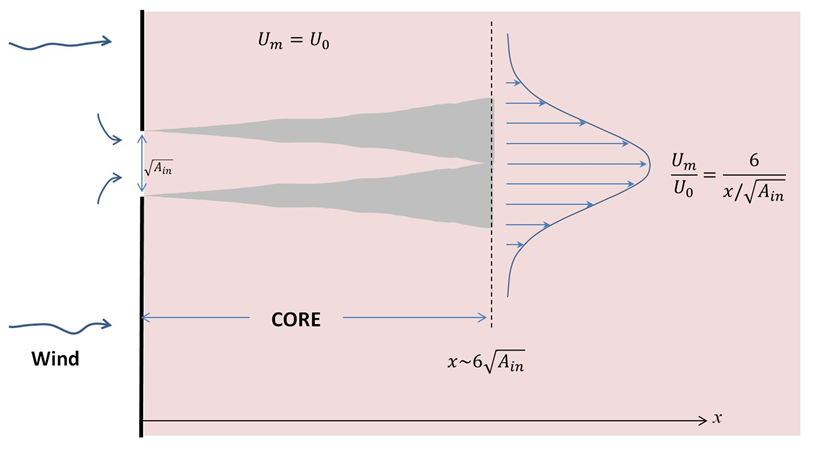
\includegraphics[width=0.9\textwidth, height=0.9\textheight, keepaspectratio=true]{media/image2622.png}
\caption{Development of an axisymmetric jet from airflow through a window. \protect \label{fig:development-of-an-axisymmetric-jet-from}}
\end{figure}

Air flows into the room through an inflow window in the form of an approximately axisymmetric jet, with characteristic diameter \emph{L} = \emph{A}\(_{in}\)\(^{1/2}\), that is confined by the room surfaces (see Figure~\ref{fig:top-view-of-a-cross-ventilated-room.-the-air}). The initial portion of the jet (up to six diameters) is called the potential core and is characterized by shear layer development along the perimeter of the jet. After this phase the jet transitions into a self similar profile whose centerline velocity decays as 1/\emph{x}', where \emph{x}' = \emph{x}/\emph{D} (Awbi, 2003).

For the relevant room length range the geometries used in the two models result in:

~~~~~ New model:~~~~~~~~~~~~~~~~~ 6~\textless{}~x'~\textless{}~60

~~~~~ Existing model: ~~~~~~~~~~~ 2~\textless{}~x'~\textless{}~18

The smaller openings used in the new model result in significantly more space for jet development along the room length. In all but the shortest rooms the jet will enter the fully developed stage characterized by a 1/\emph{x}' centerline velocity decay rate. For this reason, the updated model uses the average jet velocity profile as opposed to shear layer momentum transfer.

\subsubsection{Components of the flow}\label{components-of-the-flow}

Figure~\ref{fig:development-of-an-axisymmetric-jet-from} shows the schematic development of a free axisymmetric jet in an unconfined environment, and Figure~\ref{fig:top-view-of-a-cross-ventilated-room.-the-air} depicts the confinement effects. The air entrained by the jet is detrained at the outlet, creating two recirculation zones that do not exist in a free jet.

The recirculation flow is similar to the flow in a lid driven cavity, where here the driving force is the confined jet flow. Turbulent lid driven cavity flows have been shown to have self-similar velocity profiles, as shown in Figure~\ref{fig:top-view-of-one-half-of-a-cross-ventilated}.

The model is based on the hypothesis that the flow is composed of:

~~~~~ A -- Lid driven cavity flows (in the recirculation regions).

~~~~~ B -- A confined axisymmetric jet flow.

\begin{figure}[hbtp] % fig 137
\centering
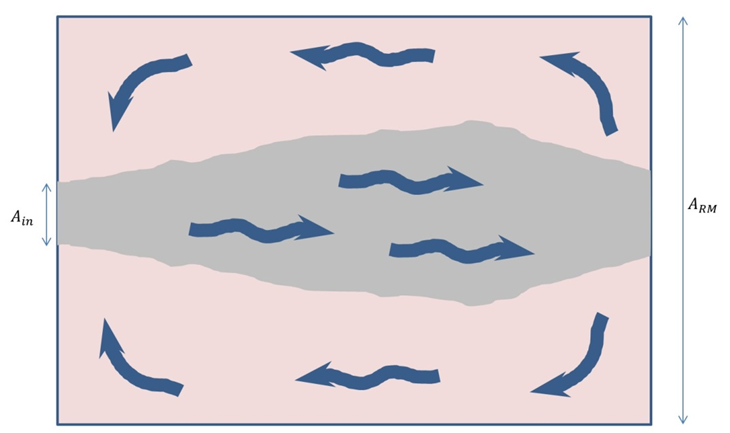
\includegraphics[width=0.9\textwidth, height=0.9\textheight, keepaspectratio=true]{media/image2623.png}
\caption{Top view of a cross ventilated room. The air entrained by the jet is detrained at the outlet, typically creating two recirculation zones. \protect \label{fig:top-view-of-a-cross-ventilated-room.-the-air}}
\end{figure}

\begin{figure}[hbtp] % fig 138
\centering
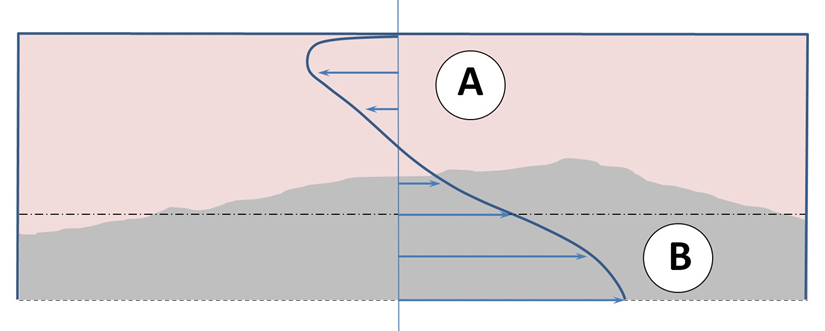
\includegraphics[width=0.9\textwidth, height=0.9\textheight, keepaspectratio=true]{media/image2624.png}
\caption{Top view of one half of a cross ventilated room. The flow is approximately composed of a confined jet and two lid driven cavity flows (one on each side). \protect \label{fig:top-view-of-one-half-of-a-cross-ventilated}}
\end{figure}

The goal of the model is to obtain the value and functional form of the constant term shown in the scaling laws for the characteristic average velocities in the two flow regions: jet and recirculation regions.

To estimate the average jet velocity we integrate along the depth of the room (including both the core region and the 1/\emph{x}' velocity decay region) to derive an average maximum jet velocity, \emph{V}\(_{J,m}\):∙

\begin{equation}
{V_{J,m}} = {U_{in}}\sqrt {{A_{in}}} \left\{ {6 + 6.3\ln \left( {{D^*}/6\sqrt {{A_{in}}} } \right)} \right\}/{D^*}
\end{equation}

(To allow for wind angle effects the room depth \emph{D} has been replaced by \emph{D}* - see a later section.) The lid-driven cavity flow profile that characterizes the recirculation region has a maximum velocity that is approximately one half of the driving velocity, which in this case is due to the jet. For this reason we define the separation between the two regions along the virtual surface where the jet reaches 50\% of its maximum, centerline, velocity.

The analysis of the flow revealed that the room containment effect leads to higher velocities for cases that combine a large inflow opening with a small room cross-section area. In order to account for this effect we propose to use the following non-dimensional scaling parameter:

\begin{equation}
{C_{RM}} = {\left( {{A_{in}}/{A_{RM}}} \right)^{1/2}}
\end{equation}

The expression used for the scaling of the average jet velocity is then:

\begin{equation}
{U_J} = {C_1}{C_{RM}}{V_{J,m}}
\end{equation}

or

\begin{equation}
{U_J} = {C_1}\frac{{{Q_{in}}}}{{\sqrt {{A_{in}}{A_{RM}}} }}\left( {{V_{J,m}}/{U_{in}}} \right)
\end{equation}

where the constant \emph{C}\(_{1}\) will be obtained from the results of a set of CFD simulations shown in the next section.

In addition to the jet velocity the characteristic recirculation flow velocity \({U_R}\) is also an interesting parameter that, according to the self-similar flow profile hypothesis shown in Figure~\ref{fig:top-view-of-one-half-of-a-cross-ventilated}, should scale with a similar expression to the one shown above for the jet (although with a different correlation constant, \emph{C}\(_{2}\)). The modeling hypothesis can also be tested by evaluating its capability to predict the maximum recirculation flow rate, which can be predicted by multiplying the average velocity by the room cross-section area:

\begin{equation}
{Q_R} = {C_3}\frac{{{Q_{in}}}}{{{C_{RM}}}}\left( {{V_{J,m}}/{U_{in}}} \right)
\end{equation}

Because of the self-similar velocity profile shape that occurs in the recirculation, the near wall velocity (used to predict forced convection) can be estimated simply by multiplying the characteristic recirculation velocity by two.

The expressions obtained apply in the turbulent regime (because the CFD simulations on which they are based are for that regime). Both velocity correlations presented below have the functional form:

\begin{equation}
V = aX + b
\end{equation}

where \emph{a} is \emph{C}\(_{1}\), \emph{C}\(_{2}\) or \emph{C}\(_{3}\), X is a velocity scale and \emph{b} is a constant that results from the best fit. The model has a lower limit on the value of \emph{X}: if \emph{X} is too small the flow is no longer turbulent. This limit implies that the point \emph{X}~ = ~0 is never achieved, avoiding the unrealistic prediction of \emph{V}(0) = \emph{b}.

In addition to the velocity and airflow rate predictions described above it is also essential to predict the temperature variations in the two zones of the flow. In most cases these variations will be positive due to the internal sensible heat gains. However`, as a result of room surface heat transfer, in some cases the variations may be negative. Analysis of the CFD simulations that are presented in the next section revealed that approximately all the exhaust air comes from the jet regions. For this reason, the heat gains affect the two regions differently:

\begin{itemize}
\item Heat gains in the jet region only affect this region (no temperature increase in the recirculation regions).
\item Heat gains in the recirculations affect both jet and recirculation regions (because they must be exhausted by the jets).
\end{itemize}

In order to predict the temperature increase, heat gains were inserted into the recirculation regions for different room geometries in the set of simulations presented in the next section. The volume containing the heat gains extended over the whole depth of the room, from floor to ceiling, and in the lateral direction from halfway between the window edge and the wall all the way to the wall. Applying energy conservation principles to predict the temperature increase in the jet and recirculation region as a function of the sensible heat gains in each region (the sum of internal gains and internal surface heat transfer) we can obtain the average value of temperature increase in each region:

\begin{equation}
\Delta {T_J} = {C_{T,J}}\frac{{q'{'_{RM}}}}{{\rho {c_p}{Q_{in}}}}
\end{equation}

\begin{equation}
\Delta {T_R} = {C_{T,R}}\frac{{q'{'_{RM}}}}{{\rho {c_p}{Q_{in}}}}
\end{equation}

where q''\(_{RM}\) is the total internal heat gain for the room, \(\rho\) and \emph{c}\(_{p}\) are the density and specific heat capacity of air, respectively, and \emph{C}\(_{T,J}\), \emph{C}\(_{T,R}\) are constants.

\subsubsection{Results}\label{results}

Table~\ref{table:test-cases-used-to-develop-correlations} lists the cases used to develop the updated CV model, which predicts the output variables defined in Table~\ref{table:definitions-of-output-variables} (see also Figure~\ref{fig:jet-and-recirculation-regions-in-typical}). Figures~\ref{fig:jet-veolicty-correlation},~\ref{fig:recirculation-region-velocity}, and~\ref{fig:recirculation-region-flow-rate} show plots of the data derived from the CFD simulations of these test cases, and the lines giving the best fit to the data. Table~\ref{table:correlation-formulae-in-the-form-y-ax-+-b} summarizes the correlation formulae and constants. Finally, Table~\ref{table:accuracy-of-correlation-formulae-in} provides estimates for the error of the correlation in each test case.

\begin{figure}[hbtp] % fig 139
\centering
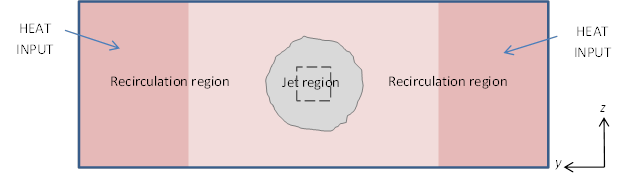
\includegraphics[width=0.9\textwidth, height=0.9\textheight, keepaspectratio=true]{media/image2634.png}
\caption{Jet and recirculation regions in typical vertical cross-section through room (y-z plane). Jet boundary occurs where jet velocity has fallen to 50\% of centerline maximum. Remainder of cross-section is treated as recirculation. Volumetric heat sources ar \protect \label{fig:jet-and-recirculation-regions-in-typical}}
\end{figure}

% table 44
\begin{longtable}[c]{@{}lllll@{}}
\caption{Test cases used to develop correlations \label{table:test-cases-used-to-develop-correlations}} \tabularnewline
\toprule 
Case & Opening area & Room width & Room depth & Room height \tabularnewline
  & A (m\(^2\)) & W (m) & D (m) & H (m) \tabularnewline

\midrule
\endfirsthead

\caption[]{Test cases used to develop correlations} \tabularnewline
\toprule 
Case & Opening area & Room width & Room depth & Room height \tabularnewline
  & A (m\(^2\)) & W (m) & D (m) & H (m) \tabularnewline

\midrule
\endhead

1 & 0.25 & 6 & 9 & 2.3 \tabularnewline
2 & 0.25 & 11 & 9 & 2.3 \tabularnewline
3 & 0.5 & 9 & 4.5 & 2.3 \tabularnewline
4 & 0.5 & 9 & 6 & 2.3 \tabularnewline
5 & 0.5 & 6 & 9 & 2.3 \tabularnewline
6 & 0.5 & 9 & 9 & 2.3 \tabularnewline
7 & 0.5 & 11 & 9 & 2.3 \tabularnewline
8 & 0.5 & 13.5 & 9 & 2.3 \tabularnewline
9 & 0.5 & 9 & 13.5 & 2.3 \tabularnewline
10 & 0.5 & 9 & 18 & 2.3 \tabularnewline
11 & 0.5 & 13.5 & 18 & 2.3 \tabularnewline
12 & 1 & 9 & 9 & 2.3 \tabularnewline
13 & 1 & 9 & 13.5 & 2.3 \tabularnewline
14 & 1 & 9 & 18 & 2.3 \tabularnewline
   & RANGE (max:min ratio) \tabularnewline
 & 4 & 2.25 & 4 & 1 \tabularnewline
\bottomrule
\end{longtable}

% table 45
\begin{longtable}[c]{p{1.25in}p{0.5in}p{0.5in}p{3.0in}}
\caption{Definitions of output variables \label{table:definitions-of-output-variables}} \tabularnewline
\toprule 
Output variable & Symbol & Units & Definition \tabularnewline
\midrule
\endfirsthead

\caption[]{Definitions of output variables} \tabularnewline
\toprule 
Output variable & Symbol & Units & Definition \tabularnewline
\midrule
\endhead
Jet velocity & U\(_J\) & m/s & Volume-averaged jet region velocity. The averaging volume is bounded at each x along the room depth by the line in the y-z plane where the jet velocity drops to 50\% of its maximum centerline value. \tabularnewline
Recirculation zone velocity & U\(_R\) & m/s & Area-averaged velocity in the y-z plane with maximum flow. The averaging area is the recirculation part of the room cross-section. Typically the plane of maximum flow occurs at x~\(\sim\)~2D/3 (D/3 before the outlet). \tabularnewline
Recirculation zone flow rate & Q\(_R\) & m\(^3\)/s & Total flow rate for the recirculation regions in the plane of maximum flow (see above). \tabularnewline
Jet temperature rise & $\Delta$T\(_J\) & °C & Volume-averaged temperature variations in the jet region, over the same volume used to define the jet velocity average. \tabularnewline
Recirculation zone temperature rise & $\Delta$T\(_R\) & °C & Volume-average temperature variations in the recirculation region. The average is calculated over the cuboidal volume placed in each recirculation containing the volumetric sensible heat gains (see main text). \tabularnewline
\bottomrule
\end{longtable}

See also Figure~\ref{fig:jet-and-recirculation-regions-in-typical}. Note the \emph{x}-coordinate is along the room, the \emph{y}-coordinate is across the room and the \emph{z}-coordinate is vertical.

% table 46
\begin{longtable}[c]{p{1.0in}p{0.5in}p{2.0in}p{0.5in}p{0.5in}p{0.5in}}
\caption{Correlation formulae in the form Y = aX + b \label{table:correlation-formulae-in-the-form-y-ax-+-b}} \tabularnewline
\toprule 
~ & Y & X & a & b & R\(^2\) \tabularnewline
\midrule
\endfirsthead

\caption[]{Correlation formulae in the form Y = aX + b} \tabularnewline
\toprule 
~ & Y & X & a & b & R\(^2\) \tabularnewline
\midrule
\endhead
Jet velocity & U\(_J\)/U\(_{in}\) & $\sqrt{A_{in}/A_{RM}} \cdot \left(V_{J,m}/U_{in}\right)$ & 1.6173 & 0.1466 & 0.8343 \tabularnewline
Recirculation zone velocity & U\(_R\)/U\(_{in}\) & $\sqrt{A_{in}/A_{RM}} \cdot \left(V_{J,m}/U_{in}\right)$ & 0.8911 & 0.0393 & 0.6464 \tabularnewline
Recirculation zone flow rate & Q\(_R\)/U\(_{in}\) & $\sqrt{A_{in}/A_{RM}} \cdot \left(V_{J,m}/U_{in}\right)$ & 0.4444 & 0.1751 & 0.6761 \tabularnewline
Jet temperature rise & $\Delta$T\(_J\) & $\frac{q''_{RM}}{\rho {c_p}{Q_{in}}}$ & 0.8254 & 0 & n/a \tabularnewline
Recirculation zone temperature rise & $\Delta$T\(_R\) & $\frac{q''_{RM}}{\rho {c_p}{Q_{in}}}$ & 1.2734 & 0 & n/a \tabularnewline
\bottomrule
\end{longtable}

% table 47
\begin{longtable}[c]{p{0.5in}p{0.4in}p{0.4in}p{0.4in}p{0.4in}p{0.4in}p{0.6in}p{0.6in}p{0.6in}p{0.6in}}
\caption{Accuracy of correlation formulae in predicting test case results \label{table:accuracy-of-correlation-formulae-in}} \tabularnewline
\toprule 
Cases & Errors (\%) \tabularnewline
\midrule
\endfirsthead

\caption[]{Accuracy of correlation formulae in predicting test case results} \tabularnewline
\toprule 
Cases & Errors (\%) \tabularnewline
\midrule
\endhead

ID & A (m2) & W (m) & D (m) & H (m) & Jet Velocity & Recirc- ulation Velocity & Recirc- ulation Flow Rate & Jet Temperature Rise & Recirc- ulation Temperature Rise \tabularnewline
1 & 0.25 & 6 & 9 & 2.3 & 16 & 45 & 60 & 1 & 10 \tabularnewline
2 & 0.25 & 11 & 9 & 2.3 & 5 & 43 & 32 & 5 & 7 \tabularnewline
3 & 0.5 & 9 & 4.5 & 2.3 & 2 & 18 & 27 & 15 & 2 \tabularnewline
4 & 0.5 & 9 & 6 & 2.3 & 6 & 32 & 28 & 7 & 1 \tabularnewline
5 & 0.5 & 6 & 9 & 2.3 & 7 & 6 & 21 & 7 & 0 \tabularnewline
6 & 0.5 & 9 & 9 & 2.3 & 10 & 4 & 6 & 15 & 17 \tabularnewline
7 & 0.5 & 11 & 9 & 2.3 & 6 & 7 & 0 & 14 & 20 \tabularnewline
8 & 0.5 & 13.5 & 9 & 2.3 & 14 & 9 & 5 & 21 & 2 \tabularnewline
9 & 0.5 & 9 & 13.5 & 2.3 & 10 & 11 & 17 & 7 & 8 \tabularnewline
10 & 0.5 & 9 & 18 & 2.3 & 10 & 25 & 29 & 8 & 3 \tabularnewline
11 & 0.5 & 13.5 & 18 & 2.3 & 8 & 2 & 23 & 9 & 6 \tabularnewline
12 & 1 & 9 & 9 & 2.3 & 2 & 5 & 3 & 3 & 4 \tabularnewline
13 & 1 & 9 & 13.5 & 2.3 & 8 & 10 & 10 & 3 & 6 \tabularnewline
14 & 1 & 9 & 18 & 2.3 & 0 & 18 & 6 & 13 & 2 \tabularnewline
Average & 8 & 17 & 19 & 9 & 6 \tabularnewline
\bottomrule
\end{longtable}

In each case the error is the percentage difference between the given correlation prediction and the test case result obtained from CFD, i.e.~100*\textbar{}(correlation prediction -- CFD)/CFD\textbar{}.

\begin{figure}[hbtp]
\centering
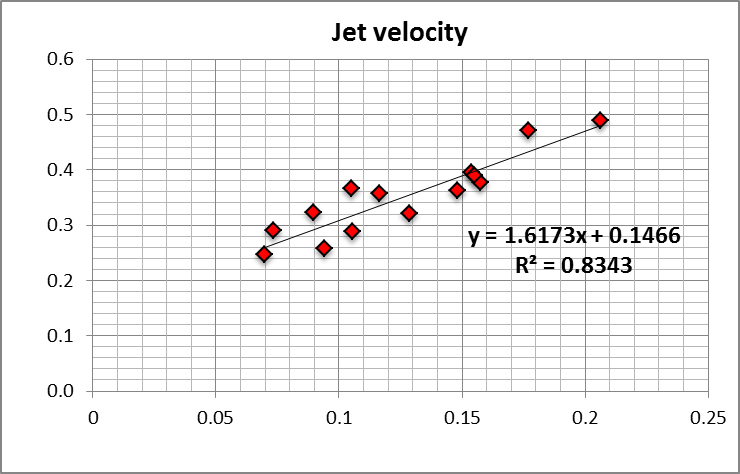
\includegraphics[width=0.9\textwidth, height=0.9\textheight, keepaspectratio=true]{media/image2652.png}
\caption{Jet velocity correlation. \protect \label{fig:jet-veolicty-correlation}}
\end{figure}

\begin{figure}[hbtp]
\centering
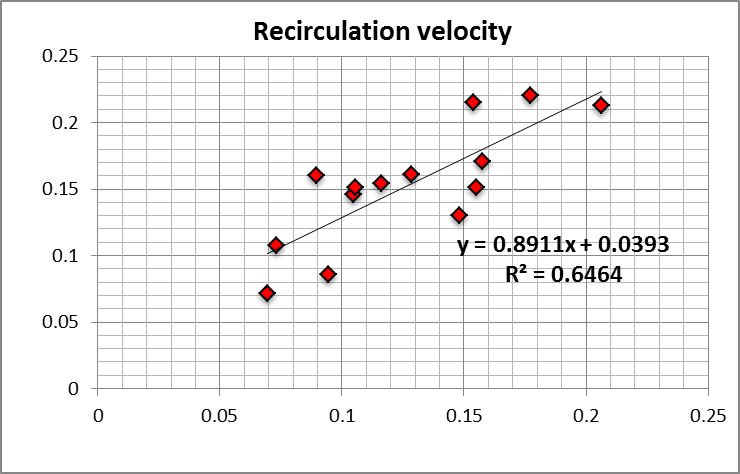
\includegraphics[width=0.9\textwidth, height=0.9\textheight, keepaspectratio=true]{media/image2655.png}
\caption{Recirculation region velocity correlation. \protect \label{fig:recirculation-region-velocity}}
\end{figure}

\begin{figure}[hbtp]
\centering
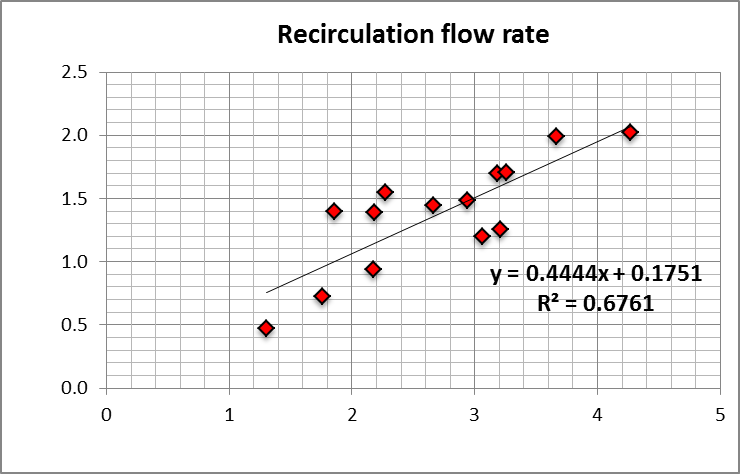
\includegraphics[width=0.9\textwidth, height=0.9\textheight, keepaspectratio=true]{media/image2658.png}
\caption{Recirculation region flow rate. \protect \label{fig:recirculation-region-flow-rate}}
\end{figure}

\subsubsection{Wind angle effects}\label{wind-angle-effects}

When the incoming wind is not normal to the façade the jet enters the room at an angle, as shown in Figure~\ref{fig:schematic-of-jet-resulting-from-wind-at-angle}.

\begin{figure}[hbtp] % fig 143
\centering
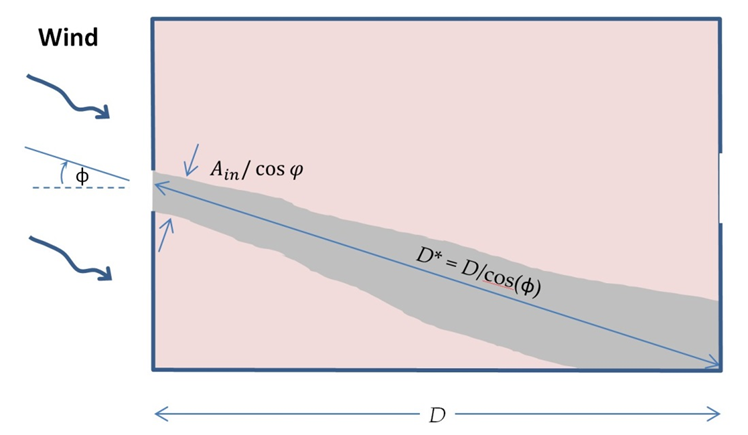
\includegraphics[width=0.9\textwidth, height=0.9\textheight, keepaspectratio=true]{media/image2659.png}
\caption{Schematic of jet resulting from wind at angle \(\phi\) to façade. \protect \label{fig:schematic-of-jet-resulting-from-wind-at-angle}}
\end{figure}

This oblique geometry has two main effects on the flow and consequent correlation predictions:

\begin{itemize}
\item The inflow area is reduced, creating a larger inflow velocity for the same flow rate.
\item The room flow path length is increased, from \emph{D} to \emph{D}*, resulting in a larger apparent depth.
\item The first effect increases indoor velocities while the second effect decreases the velocities.
\end{itemize}

\subsubsection{Multiple apertures}\label{multiple-apertures}

CFD simulations for rooms with more than one inflow aperture show that the model can be applied to these configurations with minimal adjustments. As a result of increased dissipation in the central recirculation region, where two distinct recirculation flows collide (Figure~\ref{fig:flow-regions-for-a-room-with-2-inlets-and-2}), the airflow velocities are reduced by 5-10\%, as shown in the charts in Figure~\ref{fig:jet-velocity-and-recirculation-velocity-for}.

\begin{figure}[hbtp] % fig 144
\centering
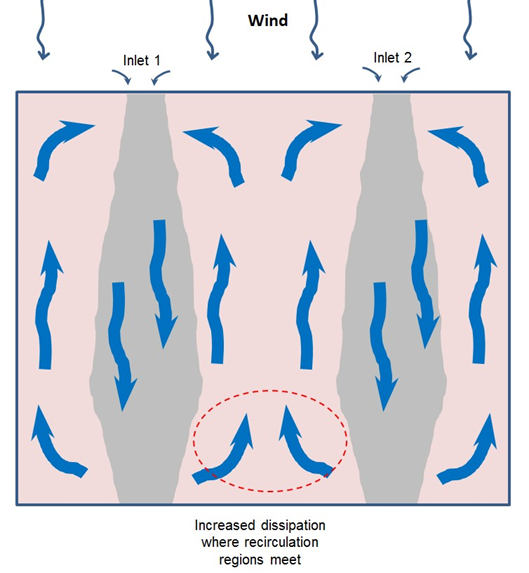
\includegraphics[width=0.9\textwidth, height=0.9\textheight, keepaspectratio=true]{media/image2660.png}
\caption{Flow regions for a room with 2 inlets and 2 outlets. \protect \label{fig:flow-regions-for-a-room-with-2-inlets-and-2}}
\end{figure}

\begin{figure}[hbtp] % fig 145
\centering
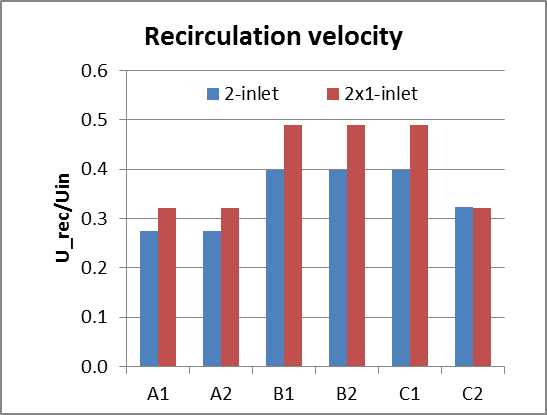
\includegraphics[width=0.9\textwidth, height=0.9\textheight, keepaspectratio=true]{media/image2662.png}
\caption{Jet velocity and recirculation velocity for the two halves of 3 different 2-inlet rooms, A-C, compared with the corresponding 1-inlet rooms. \protect \label{fig:jet-velocity-and-recirculation-velocity-for}}
\end{figure}

\textbf{\emph{Heat transfer in recirculating flows}}

In most cross ventilation flows with recirculations the mixing between recirculation and inflow jet is only partial. Figure~\ref{fig:top-view-of-the-flow-structure-in-case-r.} shows a schematic representation of the heat transfer process (showing a top view of one half of a symmetrical room). The flow is divided into three distinct streams with connected temperature variations:

\begin{itemize}
\item The main jet (labeled J in the figure).
\item The part of the recirculation flow that exchanges heat with the jet (label R).
\item The wall boundary layer part of the recirculation flow (label W).
\end{itemize}

\begin{figure}[hbtp] % fig 146
\centering
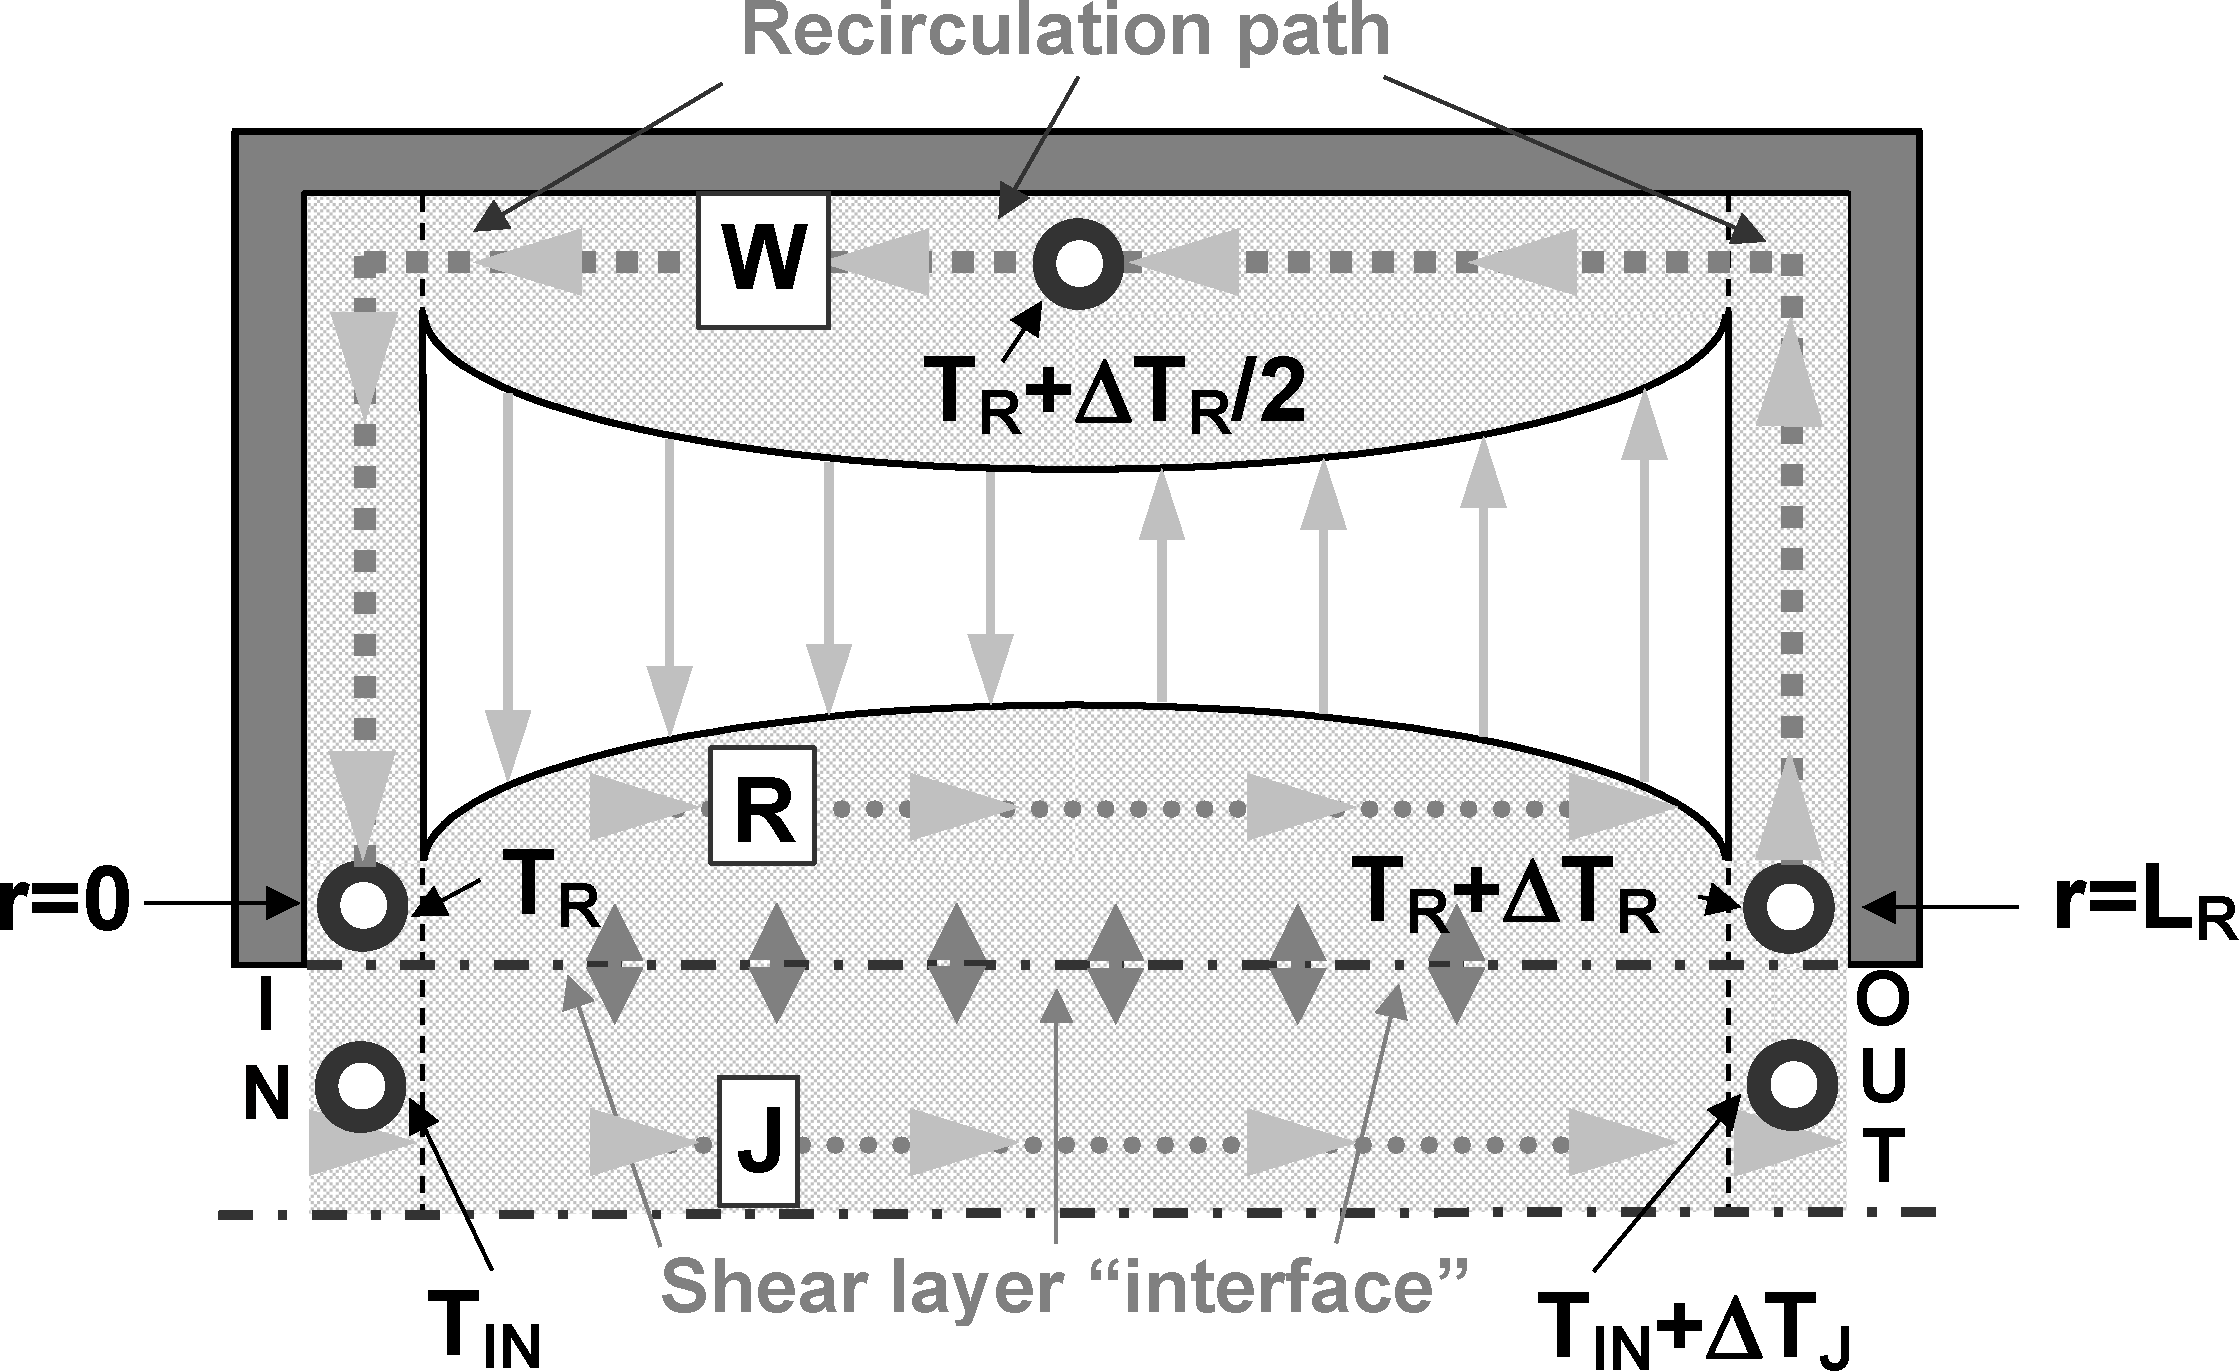
\includegraphics[width=0.9\textwidth, height=0.9\textheight, keepaspectratio=true]{media/image2663.png}
\caption{Top view of the flow structure in case R. \protect \label{fig:top-view-of-the-flow-structure-in-case-r.}}
\end{figure}

The light gray arrows show flow direction. The dark gray arrows show heat transfer in the shear layer. The recirculation region coordinate system is shown in the figure, with coordinate \emph{r} varying between 0 and \emph{L}.

\subsubsection{Heat transfer in a shear layer}\label{heat-transfer-in-a-shear-layer}

It is possible to use a formulation with a heat transfer area, a convection heat transfer coefficient and an average shear layer temperature difference to model the heat exchange between jet and recirculation flows:

\begin{equation}
{Q_{y = 0}} = {A_{SL}}{h_{SL}}\Delta {T_{SL}}
\end{equation}

\begin{equation}
{A_{SL}} = L P
\end{equation}

\begin{equation}
{h_{SL}} = \frac{{\rho \,{C_P}\,F}}{{{C_D}\,\,{A_{IN}}\,\,4\,\sigma \,\sqrt \pi }}
\end{equation}

Locally, the heat transfer process is driven by the variable, local, temperature difference:

\begin{equation}
\rho \,{C_P}\,F\,\frac{{\partial \,{T_J}(x)}}{{\partial \,x}} =  - \,\frac{{{A_{SL}}\,{h_{SL}}}}{L}\,\left( {{T_J}(x) - {T_R}(x)} \right) = \frac{{P\,\,\left( {{T_J}(x) - {T_R}(x)} \right)}}{{{C_D}\,{A_{IN}}\,4\,\sigma \,\sqrt \pi  }}
\end{equation}

\subsubsection{Predicting air temperature in the recirculation region of the flow}\label{predicting-air-temperature-in-the-recirculation-region-of-the-flow}

An accurate representation of system behavior must consider both the local heat transfer in the shear layer (varying along the \emph{x} direction, driven by the temperature profiles \emph{T\(_{J}\)(x)} and \emph{T\(_{R}\)(x)}) and the heat transfer in the wall boundary layers (with temperature \emph{T\(_{W}\)(r)}). Both transfers can be modeled using differential equations, resulting in the following system of equations:

\begin{equation}
  \begin{array}{rl}
    \rho C_p F R \frac{\partial T_W \left(r\right)}{\partial r} & = \frac{A_S h_S}{L} \left(T_S - T_W \left(r\right)\right) \\
    \rho C_p F R \frac{\partial T_R \left(x\right)}{\partial x} & = \frac{A_{SL} h_{SL}}{L} \left(T_J\left(x\right) - T_R \left(x\right)\right) \\
    \rho C_p F \frac{\partial T_J \left(x\right)}{\partial x} & = \frac{A_{SL} h_{SL}}{L} \left(T_R\left(x\right) - T_J \left(x\right)\right) 
  \end{array}
  \label{eq:DiffEqForTWrTRxTJx}
\end{equation}

The relevant boundary conditions are:

\begin{equation}
{T_W}({L_{}}) = {T_R}(0)\,,\,{T_W}(0) = {T_R}(L)\,,\,\,{T_J}(0) = {T_{IN}}
\end{equation}

The first equation in Equation~\ref{eq:DiffEqForTWrTRxTJx} models heat transfer in the wall layer. The second models the temperature variation of the portion of the recirculation flow that is in contact with the jet, it differs from the third equation only in a sign (the temperature variation in \emph{T\(_{R}\)} is symmetric to the variation in \emph{T\(_{J}\)}) and the flow rate (\emph{F\(\cdot\)R} for the recirculation and \emph{F} for the main jet). The temperature in the recirculation region is given by:

\begin{equation}
{T_W}(r) = {T_S} - ({T_S} - {T_{IN}})\,\frac{{{e^{\frac{{{h_S}\,{A_S}}}{{\rho \,{C_P}\,R\,F}}\frac{r}{{{L_{}}}}}}\,({e^{ - \frac{{{A_{SL}}\,{h_{SL}}\,(1 + R)}}{{\rho \,{C_P}\,R\,F}}}} - 1)}}{{{e^{ - \frac{{{A_{SL}}\,{h_{SL}}\,(1 + R)}}{{\rho \,{C_P}\,R\,F}}}} - {e^{\frac{{{h_S}\,{A_S}}}{{\rho \,{C_P}\,R\,F}}}}\,(1 + R) + R}}
\end{equation}

\subsubsection{Heat transfer in recirculating flows with internal gains}\label{heat-transfer-in-recirculating-flows-with-internal-gains}

Whereas surface heat transfer is an important component of room heat transfer, internal gains often dominate the room temperature field. Referring to the previously used subdivision of the room into jet and recirculation regions we can see that gains can occur exclusively in the jet region, exclusively in the recirculation region or in both regions.

\subsubsection{Heat gains in the jet region}\label{heat-gains-in-the-jet-region}

The effect of gains in the jet region on room air temperature distribution is simple to model and, within the first order accuracy goal, can be characterized as follows:

For gains occurring in the jet region (between the inlet and the room outlet) a change in inflow temperature is an adequate, conservative approximation. From energy conservation we conclude that the altered inflow temperature is given by:

\begin{equation}
{T_{ING}} = {T_{IN}} + \frac{{{G_J}}}{{\rho {C_P}F}}
\label{eq:AlteredInflowTempEquation}
\end{equation}

Gains occurring in the jet region, close to the outlet can be ignored in a first order accuracy model.

Clearly the two approaches described above are only exact when: the gains occur at the inlet and perfectly mix with the inflow jet (for the first case), or whenever the gains occur very close to the outlet (in the second case). In all other situations, the first approach provides a conservative approximation. In the model implementation in EnergyPlus the user will not define the exact location of the heat gains within each region of the flow therefore, heat gains in the jet region, are inserted in two equal parts in two separate points of the jet flow (in the room entrance and before the exit, see points r = 0 and r = L\(_{R}\) in Figure~\ref{fig:top-view-of-the-flow-structure-in-case-r.}).

\subsubsection{Heat gains in the recirculation region}\label{heat-gains-in-the-recirculation-region}

When heat gains occur in the recirculation region significant heat accumulation occurs due to the limited heat transfer ability of the shear layer. Due to this limited ability, the recirculation is partially isolated from the main jet flow and higher temperatures are generated in this region whenever heat gains are present. The concept of a global heat transfer coefficient is not applicable.

In the case of a flow in a room with adiabatic surfaces and heat gains in the recirculation region the indoor air temperatures can be predicted using the solution to the following system of equations:

\begin{equation}
  \begin{array}{rl}
    \rho C_p F R \left(T_R\left(0\right) - T_R\left(L\right)\right) & = G_R \\
    \rho C_p F R \frac{\partial T_R \left(x\right)}{\partial x} & = \frac{A_{SL} h_{SL}}{L} \left(T_J\left(x\right) - T_R \left(x\right)\right) \\
    \rho C_p F \frac{\partial T_J \left(x\right)}{\partial x} & = \frac{A_{SL} h_{SL}}{L} \left(T_R\left(x\right) - T_J \left(x\right)\right)
  \end{array}
  \label{eq:TRoTRLdTRxdTJxSystem}
\end{equation}

This system of equations differs from the system shown in Equation~\ref{eq:DiffEqForTWrTRxTJx} in several ways. Because there is no wall heat transfer there is no need to split the recirculation flow in two parts (\emph{R} and \emph{W}). The temperature increase in the recirculation flow is simply defined by the internal gains (first equation in Equation~\ref{eq:TRoTRLdTRxdTJxSystem}). The second and third equations in Equation~\ref{eq:TRoTRLdTRxdTJxSystem} model shear layer heat transfer and are similar in the two cases (Equation~\ref{eq:DiffEqForTWrTRxTJx} and Equation~\ref{eq:TRoTRLdTRxdTJxSystem}).

The recirculation flow temperature at \emph{x} = 0 is given by:

\begin{equation}
{T_R}(0) = {T_{IN}} + \left( {\frac{1}{{{e^{\frac{{{A_{SL}}{h_{SL}}\,(1 + R)}}{{\rho \,{C_P}F\,R}}}} - 1}} + 1} \right)\frac{{{G_R}(1 + R)}}{{\rho \,{C_P}F\,R}}
\end{equation}

The temperature in the recirculation is inversely proportional to the recirculation flow ratio (\emph{R}) and the shear layer area (measured by the product: \emph{A\(_{SL}\) h\(_{SL}\)}). As both of these parameters increase this expression becomes similar to Equation~\ref{eq:AlteredInflowTempEquation}. The recirculation flow temperature at \emph{x = L} is given by:

\begin{equation}
{T_R}(L) = {T_R}(0) + \Delta {T_R}
\end{equation}

The temperature variations in the recirculation flow is given by:

\begin{equation}
\Delta {T_R} = \frac{{{G_R}}}{{\rho \,{C_P}\,F\,R}}
\end{equation}

\subsubsection{Combined effects of surface heat transfer and internal gains in the recirculation region}\label{combined-effects-of-surface-heat-transfer-and-internal-gains-in-the-recirculation-region}

In this case, the following system of equations must be solved:

\begin{equation}
\begin{array}{rl}
    \rho C_p F R \frac{\partial T_W \left(r\right)}{\partial r} & = -\frac{A_S h_S}{L} \left(T_S - T_W \left(r\right)\right) - \frac{G_R}{L_R} \\
    \rho C_p F R \frac{\partial T_R \left(x\right)}{\partial x} & = \frac{A_{SL} h_{SL}}{L} \left(T_J\left(x\right) - T_R \left(x\right)\right) \\
    \rho C_p F \frac{\partial T_J \left(x\right)}{\partial x} & = \frac{A_{SL} h_{SL}}{L} \left(T_R\left(x\right) - T_J \left(x\right)\right) 
  \end{array}
\end{equation}

With the boundary conditions: \({T_W}(L) = {T_R}(0)\,,\,{T_W}(0) = {T_R}(L)\,,\,\,{T_J}(0) = {T_{IN}}\)

For simplicity the heat gains are considered to be evenly distributed along the recirculation path. The temperature variation in the recirculation region is given by:

\begin{equation}
{T_W}(r) = {T_S} + \frac{{{G_R}}}{{{A_S}\,{h_S}}} - \frac{{{e^{\frac{{{h_S}\,{A_S}}}{{\rho \,{C_P}\,R\,F}}\frac{r}{{{L_R}}}}}\,({e^{ - \frac{{{A_{SL}}\,{h_{SL}}\,(1 + R)}}{{\rho \,{C_P}\,R\,F}}}} - 1)\,({G_R} + {A_S}\,{h_S}\,({T_S} + {T_{IN}}))}}{{{e^{ - \frac{{{A_{SL}}\,{h_{SL}}\,(1 + R)}}{{\rho \,{C_P}\,R\,F}}}} + R - {e^{\frac{{{h_S}\,{A_S}}}{{\rho \,{C_P}\,R\,F}}}}\,(1 + R)}}
\end{equation}

% table 48
\begin{longtable}[c]{p{1.0in}p{1.0in}p{3.5in}}
\caption{List of variables for CV model \label{table:list-of-variables-for-cv-model}} \tabularnewline
\toprule 
Symbol & Units & Description \tabularnewline
\midrule
\endfirsthead

\caption[]{List of variables for CV model} \tabularnewline
\toprule 
Symbol & Units & Description \tabularnewline
\midrule
\endhead

a & - & Slope of correlation line of best fit \tabularnewline
A\(_{in}\) & m\(^2\) & Inlet area \tabularnewline
A\(_{RM}\) & m\(^2\) & Room cross-sectional area \tabularnewline
b & - & Intercept of correlation line of best fit \tabularnewline
c\(_{p}\) & J/kg/K & Specific heat capacity of air \tabularnewline
C\(_{RM}\) & - & Confinement scaling factor, (A\(_{in}\)/A\(_{RM}\))\(^{1/2}\) \tabularnewline
C\(_{1}\) & - & Correlation constant for jet velocity \tabularnewline
C\(_{2}\) & - & Correlation constant for recirculation velocity \tabularnewline
C\(_{3}\) & - & Correlation constant for recirculation flow rate \tabularnewline
D & m & Room depth, distance between inlet and outlet facades \tabularnewline
D* & m & Effective room depth adjusted for wind angle \tabularnewline
H & m & Room height \tabularnewline
q\(^{''}_{RM}\) & W & Total heat input from internal heat sources \tabularnewline
Q\(_{in}\) & m\(^3\)/s & Inlet flow rate, A\(_{in}\)U\(_{in}\) \tabularnewline
Q\(_R\) & m\(^3\)/s & Maximum recirculation region flow rate \tabularnewline
U\(_{in}\) & m/s & Inlet velocity, average over inlet area \tabularnewline
U\(_{m}\) & m/s & Maximum centerline velocity of jet \tabularnewline
U\(_{o}\) & m/s & Uniform inlet velocity of jet \tabularnewline
U\(_{J}\) & m/s & Volume-averaged jet velocity \tabularnewline
U\(_{R}\) & m/s & Average recirculation region velocity over plane of maximum flow \tabularnewline
V & m/s & Velocity scale \tabularnewline
V\(_{J,m}\) & m/s & Average of U\(_{m}\) over room depth \tabularnewline
W & m & Room width \tabularnewline
x & m & Coordinate along room depth, 0 $\leq$ x $\leq$ D \tabularnewline
x' & - & Non-dimensional x-coordinate, x/D \tabularnewline
X & m/s & Velocity correlation parameter \tabularnewline
Y & m & Lateral coordinate across room width \tabularnewline
Z & m & Vertical coordinate \tabularnewline
$\Delta$T\(_{J}\) & °C & Average jet temperature variation \tabularnewline
$\Delta$T\(_{R}\) & °C & Average recirculation region temperature variation \tabularnewline
r & kg/m\(^3\) & Density of air \tabularnewline
$\phi$ & ° & Wind direction relative to façade normal \tabularnewline
\bottomrule
\end{longtable}

\subsection{RoomAirflowNetwork Model}\label{roomairflownetwork-model}

\subsubsection{Overview}\label{overview-4-001}

The RoomAirflowNetwork integrates the RoomAir model with the AirflowNetwork model. The model allows multiple Room Air nodes to be associated with AirflowNetwork intra zone nodes. The AirflowNetwork intra zone linkages provide links among the intra zone nodes and users may specify airflow components among these links. The AirflowNetwork model calculates airflows of the links. The incoming airflows are part of the zone heat and moisture balances of intra zone nodes. The model also allows users to specify a node to be connected to surfaces to have convective heat transfer and/or moisture transfer between surfaces and the node, portion of internal gains and supply air and return air fractions from zone equipment and AirLoop terminals.

The input object RoomAirSettings:AirflowNetwork lists multiple RoomAirflowNetwork nodes in a zone. The input object of RoomAirflowNetwork:Node defines a list of connections assigned to a particular RoomAirflowNetwork node so that the connections will be used as components of node heat and moisture balance equations. In addition, the input objects AirflowNetwork:IntraZone:Node and AirflowNetwork:IntraZone:Linkage specify airflow nodes, linkages, and associated flow components, so that the AirflowNetwork model is used to calculate intrazone linkage airflows, which will be a part of loads for the RoomAir node balances.

\subsubsection{Model description}\label{model-description-3-001}

The model calculates each component of the governing equations first. Then heat and moisture balance equations are solved to get the node temperature and humidity ratio at the current time step.

Governing equations for each RoomAirflowNetwork node are described below:

Energy balance equation

\begin{equation}
\begin{split}
{F_i}{C_{z,i}}\frac{{d{T_{z,i}}}}{{dt}} =& \sum\limits_{j = 1}^{{N_{i,g}}} {{F_{gain,j}{\dot Q}_{i,j}}}  + \sum\limits_{j = 1}^{{N_{i,sur}}} {{h_{i,j}}} {A_j}\left( {{T_{s,j}} - {T_{z,i}}} \right) + \sum\limits_{j = 1}^{{N_{i,AFN}}} {{{\dot m}_{AFN i,j}}} {C_p}\left( {{T_{z,j}} - {T_{z,i}}} \right)\, \\
&+ \sum\limits_{j = 1}^{{N_{i,HVAC}}} {{{F_{HVAC,j}}{\dot m}_{sup,i,j}}} {C_p}\left( {{T_{sup_j}} - {T_{z,i}}} \right)
\end{split}
\end{equation}

where:

F\(_{i}\) = Fraction of zone air volume for the ith node, defined in the Fraction of Zone Air Volume field of the RoomAir:Node:Airflownetwork

C\(_{z,i}\) = Volumetric heat capacity for the ith node: \(\rho_{air,i}\)V C\(_{p}\)C\(_{T}\)

\(\rho_{air,i}\) = Dry air density at the ith zone node

C\(_{p}\) = zone dry air specific heat

C\(_{T}\) = sensible heat capacity multiplier (Detailed description is provided below)

V = Zone air volume

T\(_{z,i}\) = Air temperature at the ith zone RoomAir node

N\(_{i,g}\) = The number of internal gains for the ith node, defined in the RoomAir:Node:Airflownetwork:InternalGains object

F\(_{gain,j}\) = Fraction of internal gain from jth internal gain object defined in the RoomAir:Node:Airflownetwork:InternalGains object

\({\dot Q}_{i,j}\) = The amount of internal sensible gain at the jth internal gain object and ith node.

\({\sum\limits_{j = 1}^{N_{i,g}} F_{gain,j}{\dot Q}_{i,j}}\) = The total amount of internal sensible gains assigned to the ith node

N\(_{i,sur}\) = The number of adjacent surface with convective heat transfer for the ith node, defined in the RoomAir:Node:Airflownetwork:AdjacentSurfaceList object

h\(_{i,j}\) = Heat transfer coefficient between the jth adjacent surface and ith node

A\(_{j}\) = Area of the jth adjacent surface

T\(_{s,j}\) = Inside temperature at the jth adjacent surface

\({\sum\limits_{j = 1}^{N_{i,sur}} h_{i,j} A_j \left( T_{s,j} - T_{z,i}\right)}\) = The total amount of convective gains from adjacent surfaces attached to the ith node

N\(_{i,AFN}\) = The number of RoomAir:Node:Airflownetwork objects connected to the ith node. The links are defined in AirflowNetwork:IntraZone:Linkage objects.

\({\dot m}_{AFN,i,j}\) = Mass flow rate from the jth node to the ith node. The flow rates are calculated in the AirflowNetwork model. It should be pointed out that the outgoing flows from the ith node will not be used in the present energy and moisture balance calculations, because they are a part of energy and moisture balances.

T\(_{z,j}\) = Air temperature at the jth zone RoomAir node

\({\sum\limits_{j = 1}^{N_{i,g}} \dot m_{AFN i,j} {C_p}\left( T_{z,j} - T_{z,i} \right)}\) = The total amount of heat transfer driven by intra zonal flows

N\(_{i,HVAC}\) = The number of RoomAir:Node:Airflownetwork:HVACEquipment objects which provide supply air to the ith node.

F\(_{HVAC,j}\) = Fraction of output or supply air to the ith node from jth HVAC equipment defined in RoomAir:Node:Airflownetwork:HVACEquipment objects

\({\dot m}_{sup,i,j}\) = The supply mass flow rate from the jth HVAC equipment

T\(_{sup,j}\) = Supply air temperature at the jth HVAC equipment

\({\sum\limits_{j = 1}^{N_{i,HVAC}} F_{HVAC,j} \dot m_{sup,i,j} \left( T_{sup,j} - T_{z,i}\right)}\) = The total amount of heat transfer from HVAC equipment to the ith node

Moisture balance equation

\begin{equation}
\begin{split}
{F_i}{M_{z,i}}\frac{{d{W_{z,i}}}}{{dt}} =& \sum\limits_{j = 1}^{{N_{i,g}}} {{F_{gain,j}{\dot Q}_{i,j}}}  + \sum\limits_{j = 1}^{{N_{i,sur}}} {{h_{M,j}}} {A_j}\left( {{W_{s,j}} - {W_{z,i}}} \right) + \sum\limits_{j = 1}^{{N_{i,AFN}}} {{{\dot m}_{AFN i,j}}} \left( {{W_{z,j}} - {W_{z,i}}} \right)\, \\
&+ \sum\limits_{j = 1}^{{N_{i,HVAC}}} {{{F_{HVAC,j}}{\dot m}_{sup,i,j}}} \left( {{W_{sup_j}} - {W_{z,i}}} \right)
\end{split}
\end{equation}

where:

Fi = Fraction of zone air volume for the ith node, defined in the Fraction of Zone Air Volume of the RoomAir:Node:Airflownetwork

M\(_{z,i}\) = Mass for the ith node: \(\rho_{air,i}\)V\(_{Cp}\)C\(_{T}\)

\(\rho_{air,i}\) = Dry air density at the ith zone RoomAir node

V = Zone air volume

W\(_{z,i}\) = Air humidity ratio at the ith zone RoomAir node

N\(_{i,g}\) = The number of internal gains for the ith node, defined in the \\ RoomAir:Node:Airflownetwork:InternalGains object

F\(_{gain,j}\) = Fraction of internal gain from jth internal gain object defined in the RoomAir:Node:Airflownetwork:InternalGains object

\({\dot Q}_{i,j}\) = The amount of internal latent gain at the jth internal gain object and ith node.

\({\sum\limits_{j = 1}^{N_{i,g}} F_{gain,j}{\dot Q}_{i,j}}\) = The total amount of internal latent gains attached to the ith node

N\(_{i,sur}\) = The number of adjacent surface with convective heat transfer for the ith node, defined in the RoomAir:Node:Airflownetwork:AdjacentSurfaceList object

h\(_{M,j}\) = Mass transfer coefficient between the jth adjacent surface and ith node

A\(_{j}\) = Area of the jth adjacent surface

W\(_{s,j}\) = Inside humidity ratio at the jth adjacent surface

\({\sum\limits_{j = 1}^{N_{i,sur}} h_{M,j} A_j \left( W_{s,j} - W_{z,i}\right)}\) = The total amount of convective moisture gains from adjacent surfaces attached to the ith node

N\(_{i,AFN}\) = The number of RoomAir:Node:Airflownetwork objects connected to the ith node. The links are defined in AirflowNetwork:IntraZone:Linkage objects.

\({\dot m}_{AFN,i,j}\) = Mass flow rate from the jth node to the ith node. The flow rates are calculated in the AirflowNetwork model. It should be pointed out that the outgoing flow from the ith node will not be used in the present calculation, because they are a part of energy balance.

W\(_{z,j}\) = Air humidity ratio at the jth zone RoomAir node

\({\sum\limits_{j = 1}^{N_{i,AFN}} \dot m_{AFN,i,j} \left( W_{z,j} - W_{z,i}\right)}\) = The total amount of moisture transfer driven by intra zonal flows

N\(_{i,HVAC}\) = The number of RoomAir:Node:Airflownetwork:HVACEquipment objects which provide supply air to the ith node.

F\(_{HVAC,j}\) = Fraction of output or supply air to the ith node from jth HVAC equipment defined in RoomAir:Node:Airflownetwork:HVACEquipment objects

\({\dot m}_{sup,i,j}\) = The supply mass flow rate from the jth HVAC equipment

W\(_{sup,j}\) = Supply air humidity ratio at the jth HVAC equipment

\({\sum\limits_{j = 1}^{N_{i,HVAC}} F_{HVAC,j} \dot m_{sup,i,j} \left( W_{sup,j} - W_{z,i}\right)}\) = The total amount of moisture transfer from HVAC equipment to the ith node

\subsubsection{Calculation procedures}\label{calculation-procedures}

The AirflowNetwork model is called first to calculate intrazone linkage air flows based on node temperatures and humidity ratios at the previous time step. The linkage loads are summarized based on each node with all incoming airflow, while any outgoing airflows from the node of the interest are excluded in the node energy and moisture balances. When the RoomAirModelAirflowNetowrk module is called, it summarizes internal gains at each node based on specification provided in the RoomAirflowNetwork:Node:InternalGains object, convective heat transfer from adjacent walls specified in the RoomAirflowNetwork:Node:AdjacentSurfaceList object. These load components are used in the predictor to predict system loads based on thermostat setpoint and supply fraction in the controlled zone node. In the corrector, the supply air conditions defined in the RoomAirflowNetwork:Node:HVACEquipment object are added. After all load components are assembled together, the node energy and moisture balance equations are solved. The node temperature and humidity ratio are calculated at the current time step.

\subsection{References}\label{ra-references}

Altmayer, E.F., Gadgil, A.J., Bauman, F.S., Kammerud, R.C. Correlations for convective heat transfer from room surfaces. ASHRAE Transactions, No. 2764.

Awbi, H.B. 2003. Ventilation of Buildings (2\textsuperscript{nd} Edition). Routledge.

Awbi, H.B. and Hatton, A. 1999. Natural convection from heated room surfaces, Energy and Buildings, 30, 233-244.

Awbi, H.B. and Hatton, A. 2000. Mixed convection from heated room surfaces, Energy and Buildings, 32, 153-166.

Aynsley, R.M., Melbourne, W., Vickery, B.J. 1977. Architectural Aerodynamics. Applied Science London.

Baturin, V. V. , Billington, N. S. 1972. Fundamentals of Industrial Ventilation, Franklin Book Company 1972, pp.~174-179.

Bejan, A. 1994. Convection Heat Transfer 2nd ed, Wiley, USA.

Carrilho da Gra\c{c}a, G. 2003. Simplified models for heat transfer in rooms. Ph. D. Thesis, University of California, San Diego.

Chandra, S., Kerestecioglu, A.A. 1984. Heat transfer in naturally ventilated rooms data from full-scale measurements, ASHRAE Transactions, Volume 90, part 1b 211-224.

Chen, Q., and B. Griffith. 2002. Incorporating Nodal Room Air Models into Building Energy Calculation Procedures. ASHRAE RP-1222 Final Report.

Cooper, P. and P.F. Linden. 1996. Natural ventilation of an enclosure containing two buoyancy sources. Journal of Fluid Mechanics, Vol. 311, pp.~153-176.

Dominique, M. and P. Guitton. 1997.~ Validation of displacement ventilation simplified models. Proc. of Building Simulation.

Griffith, B. and Q. Chen. 2004. Framework for coupling room air models to heat balance load and energy calculations (RP-1222). International Journal of Heating, Ventilating, Air-conditioning and Refrigerating Research. ASHRAE, Atlanta GA.~ Vol 10. No 2. April 2004.

Holford, J.M., G.R. Hunt and P.F. Linden. 2002. Competition between heat sources in a ventilated space. Proceedings of RoomVent 2002, pp.~577-580.

Hunt, G.R., J.M. Holford and P.F. Linden. 2002. Characterization of the flow driven by a finite area heat source in a ventilated enclosure. Proceedings of RoomVent 2002, pp.~ 581-584.

Hunt, G.R. and P.F. Linden. 2001. Steady-state flows in an enclosure ventilated by buoyancy forces assisted by wind. . Journal of Fluid Mechanics, Vol. 426,~ pp.~355-386.

Kalema, T., Haapala, T. `995. Effect of interior heat transfer coefficients on thermal dynamics and energy consumption, Energy and Buildings 22 (2) pp.~101-113.

Kaye, K.N. and P.F. Linden.~ 2004. Coalescing axisymmetric turbulent plumes\emph{.} Journal of Fluid Mechanics, ~Vol. 502, pp.~41--63.

Lin, Y.J. and P.F. Linden. 2005. A model for an under floor air distribution system. Energy\&Building, Vol. 37, pp.~399-409.

Linden, P.F., G.F. Lane-Serff and D.A. Smeed. 1990. Emptying filling boxes: the fluid mechanics of natural ventilation. Journal of Fluid Mechanics, Vol. 212, pp.~309-335.

Linden, P.F. and P. Cooper. 1996. Multiple sources of buoyancy in a naturally ventilated enclosure. Journal of Fluid Mechanics, Vol. 311, pp.~177-192.

Liu, Q. 2006. The Fluid Dynamics of an Underfloor Air Distribution System. A PhD dissertation in Engineering Sciences (Systems Science) at UC San Diego.

Morton, B.R., G.I. Taylor andJ.S. Turner. 1956. Turbulent gravitational convection from maintained and instantaneous sources. Proceedings of the Royal Society of London, Vol A234, pp.~1-23.

Mundt, E. 1996. The Performance of Displacement Ventilation Systems -- Experimental and Theoretical Studies, Ph. D. Thesis, Bulletin N38, Building Services Engineering KTH, Stockholm.

Neiswanger, L., Johnson, G.A., Carey, V.P. 1987. An experimental study of high Raleigh number mixed convection in a rectangular enclosure with restricted inlet and outlet openings. Transactions of ASME, Vol. 109, 446-453.

Ohba, M., Irie, K., Kurabuchi, T. 2001. Study on airflow characteristics inside and outside a CVmodel, and ventilation flow rate using wind tunnel experiments. Journal of Wind Engineering and Industrial Aerodynamics, in press.

Rees, S.J., and P. Haves. 2001. A nodal model for displacement ventilation and chilled ceiling systems in office spaces. Building and Environment, Vol. 26, pp.~753-762.

Siebers, D. L., Schwind, R. G., Moffat, R. J. 1983. Experimental Mixed Convection Heat Transfer From a Large Vertical Surface in a Horizontal Flow. SAND 83-8225, Sandia National Laboratories, Livermore CA.

Spitler, J. D., Pedersen, C.O., Fisher, D.E. 1991. Interior Convective Heat Transfer in Buildings with Large Ventilative Flow Rates. ASHRAE Transactions, Vol. 97, Pt.1, pp.~505-515.



